\label{chap:development}
\section{Data}

Only a limited amount of data has been provided by the company \textit{TraceParts} due to 
confidentiality. 
However, provided data has been enough to develop a methodology for, at least, a proof of concept. 
To be more specific about the provided dataset, 100 database instances have been accessed and loaded 
into the local machine environment. For this purpose, docker container(s) has been used to abstract 
the database service(s).

% \begin{figure}[H]
% 	\centering
% 	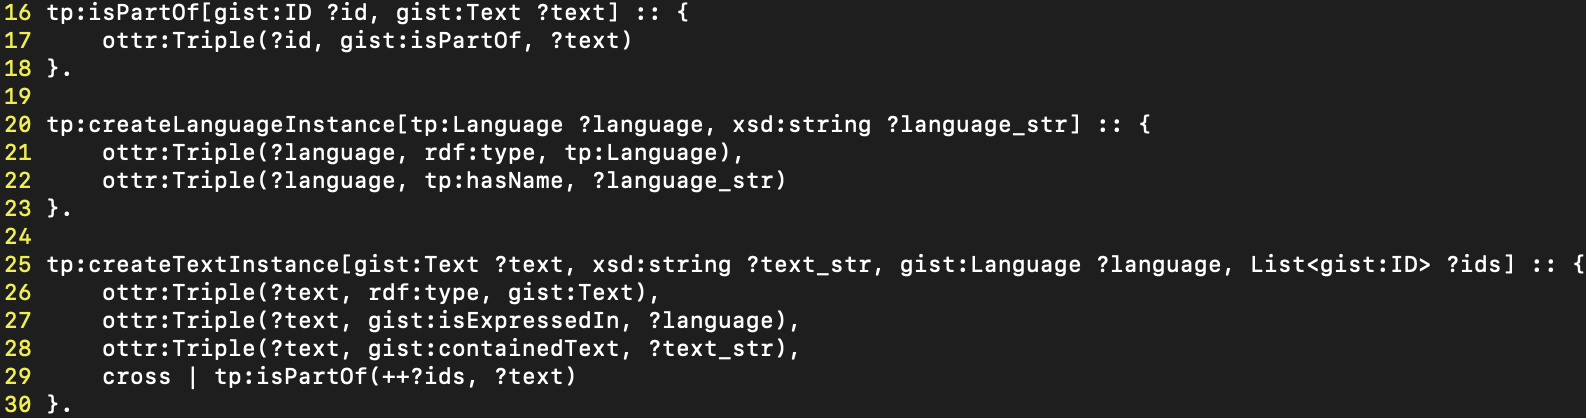
\includegraphics[width=0.75\textwidth]{../../resources/ottr_lib_example.png}
% 	\caption{ElasticSearch example}
% 	\label{fig:es_example}
% \end{figure}

\textit{ElasticSearch} (ES) is an open-source RESTful search and analytics engine which works in a 
distributed manner under the hood. It has been developed with Java and is based on Apache Lucene. 
In the ES database, data is stored with corresponding indices, and to retrieve it, we can send queries 
to its ``\lstinline{_search}'' endpoint. ES has many built-in functionalities such as filtering, 
ranking, aggregating, etc. However, we do not use any such functionalities in this project work since 
what we have been trying to achieve is a stand alone PoC system that contains all the necessary 
and customized functionalities for our use case.

\subsection{Database Schema}

The database has a somewhat complicated schema, however, there are several fields of interest for the 
matter of this internship. These fields include \textit{Part Family}, \textit{Part Number}, 
\textit{Part Family Name}, and \textit{Part Number Name}.

In the current version of the database used by the company, there are fields with the same values 
that are repeated in several places in the database memory. Such use of the service is probably 
inefficient in terms of memory complexity and maybe processing as well. In either case, there is 
inefficiency in the schema design.

\begin{table}[H]
	\centering
	\begin{tabular}{|p{0.25\textwidth}|p{0.20\textwidth}|p{0.23\textwidth}|p{0.23\textwidth}|}
		\hline
		\textbf{PartFamily} & \textbf{PartNumber} & \textbf{PartFamilyName} & \textbf{PartNumberName} \\
		\hline
		10-05112010-061898 & NSYMR34 & Telequick Mounting plate & Telequick Mounting plate 300X400 \\
		10-07032014-070631 & KTC2500ET32B & KT 3X2500CO FEEDER & KT 3X2500CO FEEDER LENGTH \\
		10-07032014-069644 & KTC1000lP7C1 & KT 5X1000CO FLAT ELBOW N1 & KT 5X1000CO FLAT ELBOW N1 \\
		10-19032018-083391 & LC1D12W7 & Contactor & Contactor - LC1D12W7 \\
		\hline
	\end{tabular}
	\caption{Example database instances}
	\label{tab:example_db_instances}
\end{table}

\section{Methods}

To make the TraceParts' search engine more semantic, the proposed solutions assume the existence of 
knowledge graph of database entities where there are relevant and useful semantic linkages between 
them. Since there is no such KG, I have proposed and implemented several solutions to fulfill this 
requirement. More specifically, I have worked on the Knowledge Acquisition part. The figure below 
illustrates the already-existing architecture of Knowledge Acquisition.

\begin{figure}[H]
	\centering
	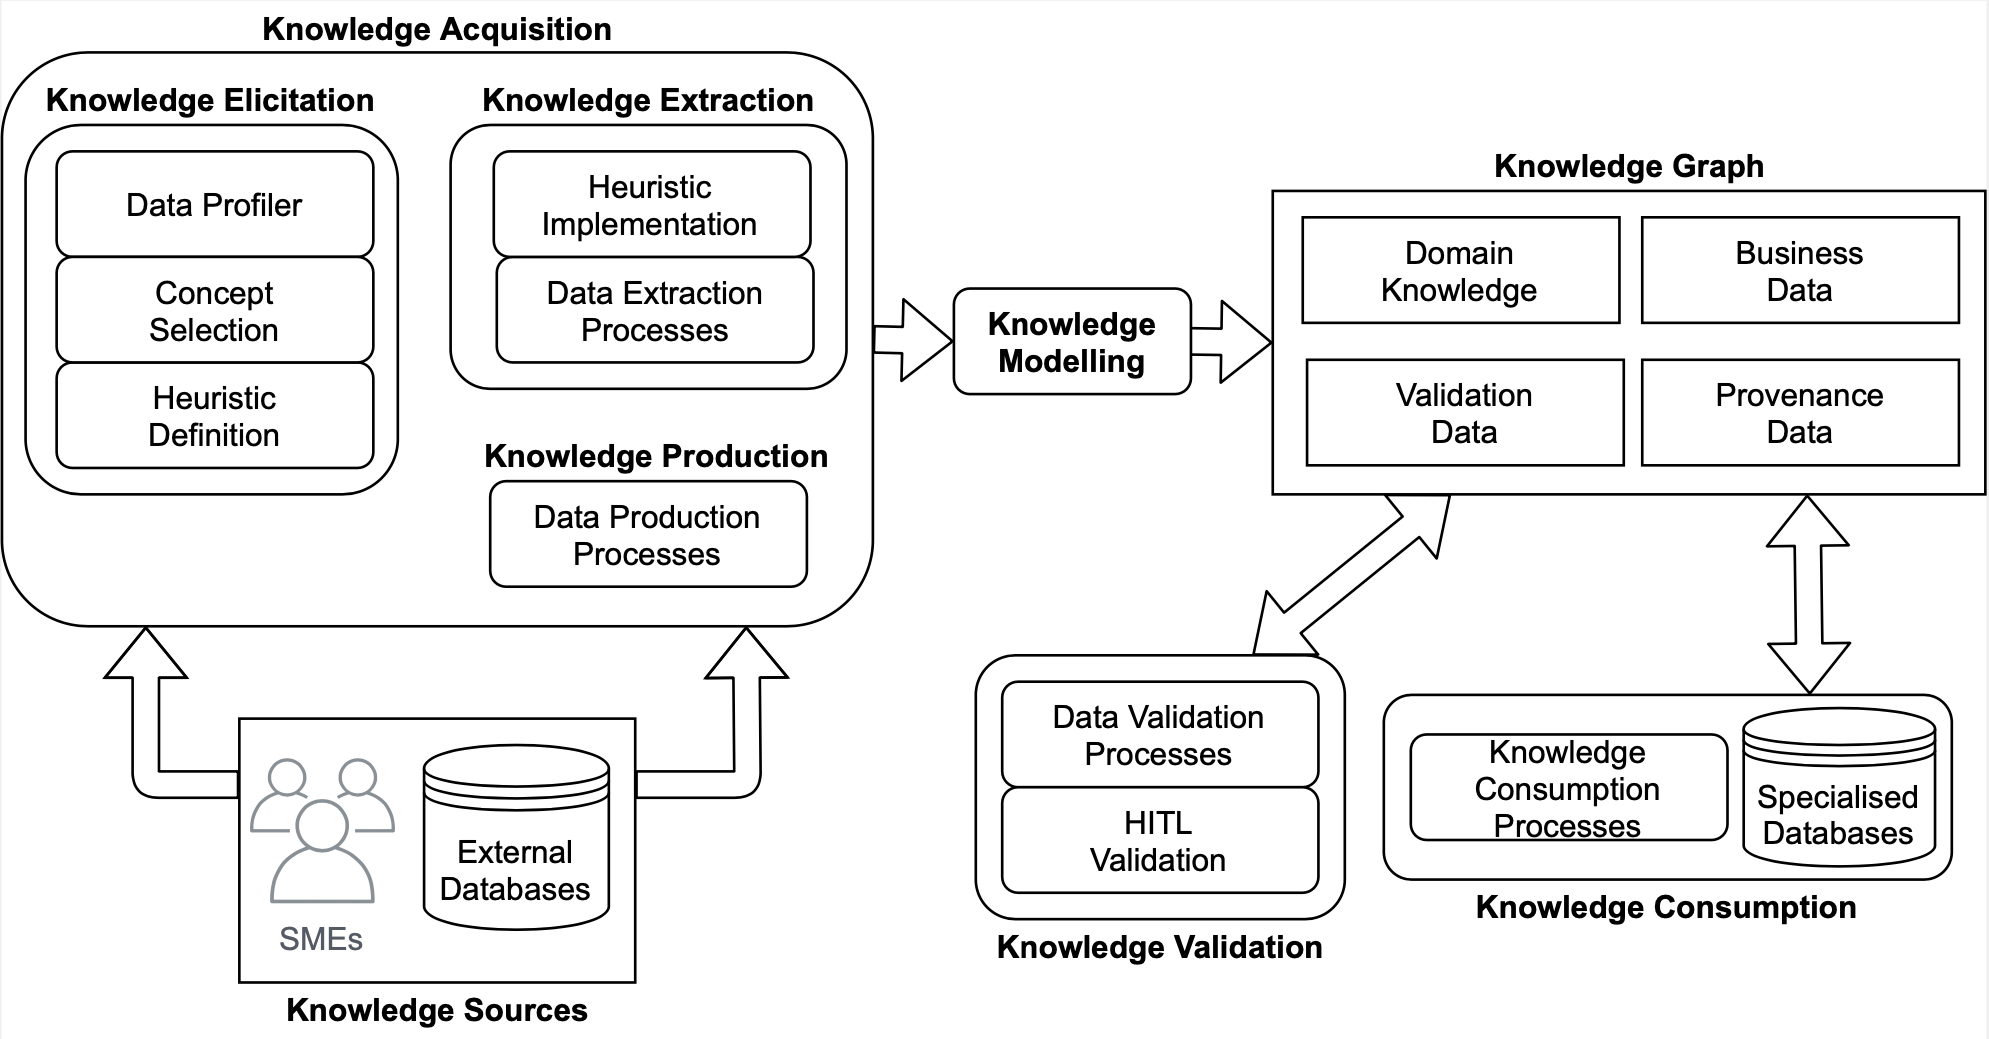
\includegraphics[width=0.75\textwidth]{../../resources/responding_pipeline.png}
	\caption{Knowledge Acquisition pipeline}
	\label{fig:responding_knowledge_acquisition_pipeline}
\end{figure}

In this figure, round-shaped rectangular boxes indicate the processes and sharp-shaped boxes indicate 
the storage. \textit{Knowledge elicitation}, \textit{knowledge extraction}, and \textit{knowledge 
consumption} are the three parts of the knowledge acquisition process.

Knowledge elicitation is the process of acquiring tacit knowledge from domain experts in the formal 
form. Conversion of tacit knowledge or insights into tangible and structured data is not trivial 
work and needs to be dealt with at the very first step of the project. 
Knowledge extraction is the process of extracting knowledge from (un)structured data containers. As 
an example of such a process, \textit{Extract-Transform-Load} (\textit{ETL}) can be given where data 
is extracted from one or more databases, then transformed in some specific way to be suitable for 
further use, and finally, loaded into one or more databases.
Knowledge production and consumption processes define how the linked data points are produced and 
requested by the end-users respectively. 

Knowledge validation is the process of KB\footnote{Knowledge Base} verification and 
evaluation \cite{LAUR,Owoc1999}. Knowledge verification focuses on the structural correctness of 
knowledge bases whereas evaluation takes care of the inference part so that only correct conclusions 
can be made within the knowledge base. There are several approaches for KB verification that are 
based on dependency tables, decision trees, machine learning, graphs, etc., and another set of 
approaches for evaluation is aimed at refinement, testing, generating, and so on.

Knowledge sources are where we acquire knowledge. These sources can either be subject-matter 
experts (SMEs) or some external databases. In the case of this project, we have used TraceParts' 
ElasticSearch database to extract knowledge, transform it to make it comply with the developed 
ontology, and load it into the Jena graph database. Throughout the rest of the processes, the only 
knowledge source has been the KG that we have acquired. This also helps us to simplify the 
knowledge validation steps since we only consider our KG as a unified source of truth and every other 
process, if needed, is built on top of this single knowledge source.

A knowledge graph is a data structure that represents some specific piece of knowledge by using 
graphs. In the context of KGs, nodes or vertices of the graph represent the concepts while edges or 
arcs represent the relationships between them. The distinction between ontologies and knowledge graphs 
is not still clear among many people. According to some sources, ontologies are only to represent 
concepts 
and relationships between those concepts whereas knowledge graphs also incorporate individuals or 
instances. However, this definition is also controversial among some other sources; for example, 
an ontology can also incorporate individuals or objects according to \cite{enwiki:1085831526}.

Although there are many debates on definitions of ontologies and knowledge graphs, I think that it may 
be a bit deviating route to take to define something whose whole purpose, ironically, is to define things. 
The reason behind this thought is that I do not think that every ``thing'' is clearly and rigorously 
definable. For example, even the concept of a ``straight line'' is not rigorously definable in the 
sense 
that its definition would not contain the concept of a straight line, or in other words, if circular 
definitions were not allowed then defining a ``straight line'' would not be possible at all and that is 
the reason it is accepted as a \textit{primitive} which is accepted to have no definition 
\cite{enwiki:1092767429}. The deeper reason for such things to happen, I think, is due to the nature of 
the language itself. We use language to describe or communicate our thoughts, feelings, emotions or 
experiences and these experiences are not inherently captured by the language itself. In fact, language is 
invented and learned by humans through an iterative process.

\subsection{Ontology Concerning The Search Engine}

The first important part of knowledge acquisition is to have an ontology describing the concepts and 
relationships between them in a formal way so that there is an agreed-upon structure of data. Developing 
an ontology is not an as easy job as it may sound. While designing an ontology, the designer should be 
aware of the implications of his/her design choices. Moreover, it is not a trivial task to be able to 
identify necessary and sufficient ontological objects (i.e, concepts and relationships). An ontology is 
considered well-designed if it is able to say what it is supposed to say and not say what it is not 
supposed to say. There is a balance between being less expressive to the degree that one cannot 
represent what is essential and more expressive to the degree that one can express a lot of things that 
are not meant to be essential. Either case is not considered good practice, in fact, it is the thin 
line that one should try to establish for the developed ontology \cite{cmariakeet}.

\begin{figure}[ht]
	\centering
	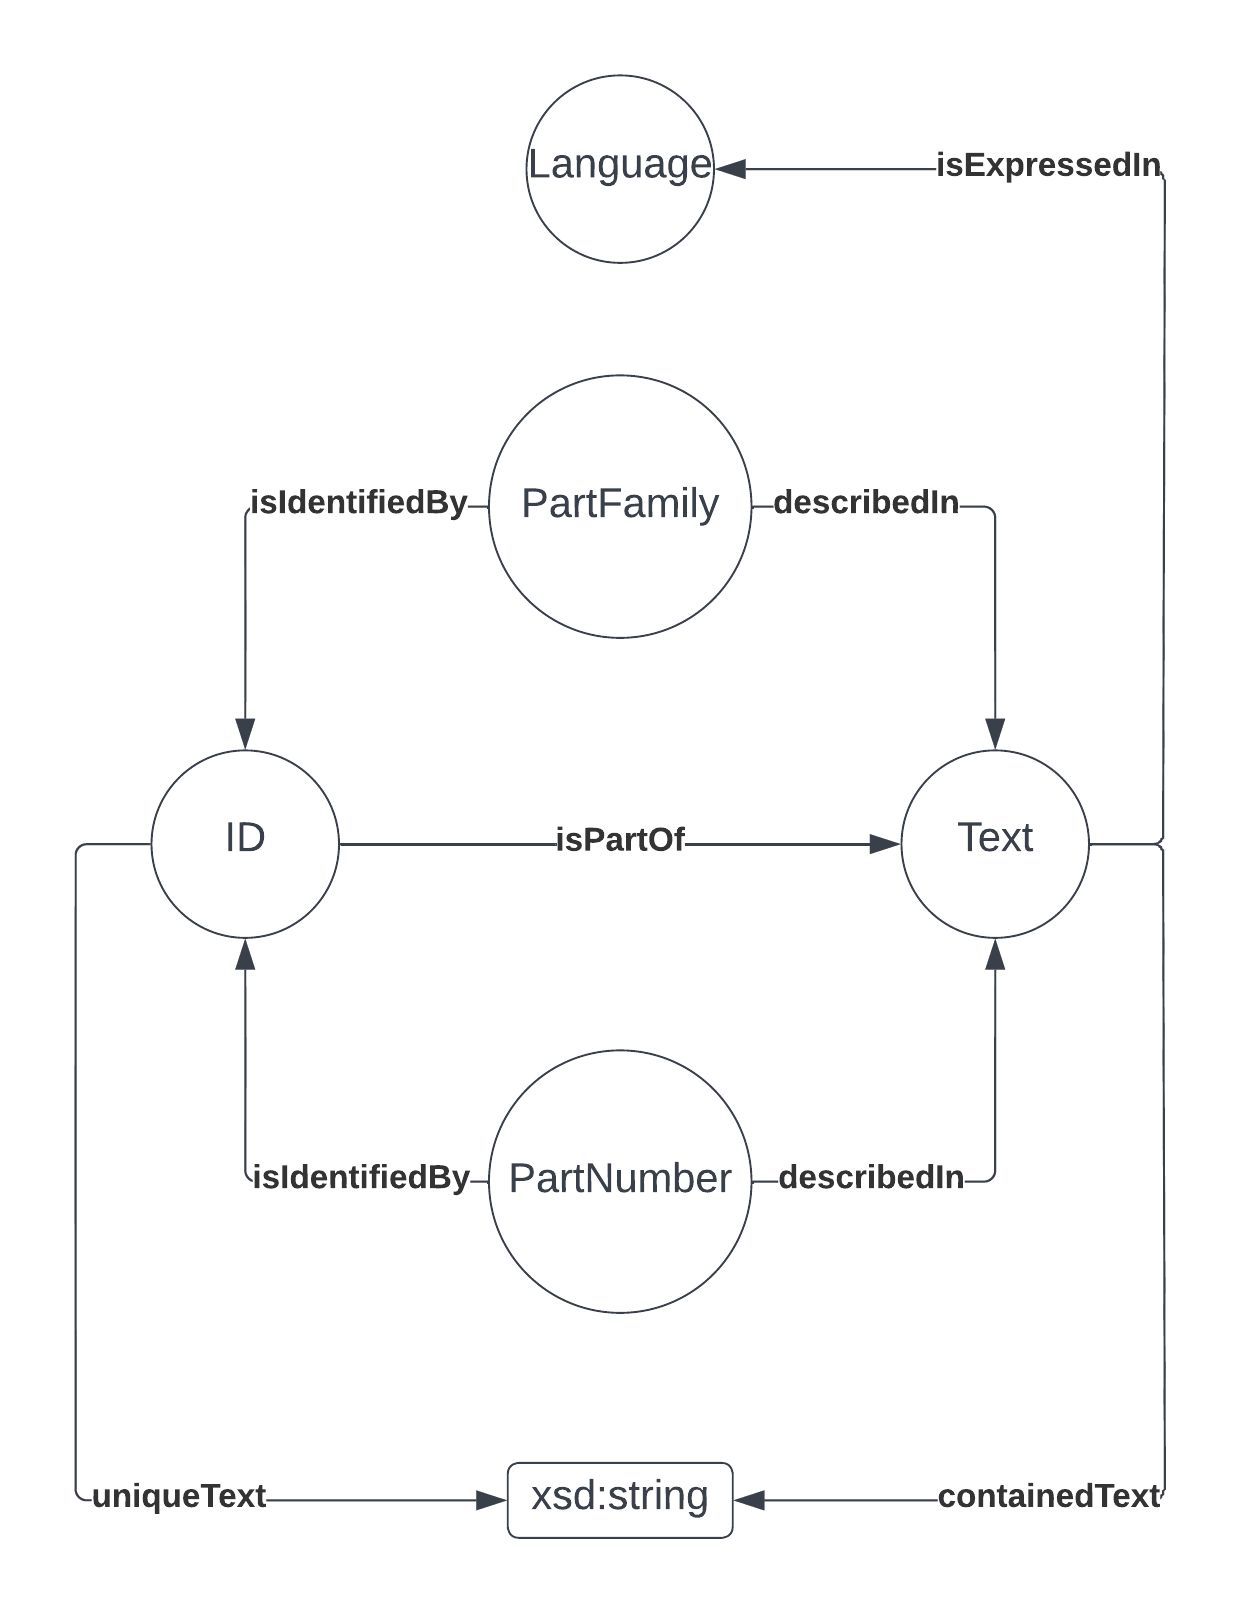
\includegraphics[width=0.70\textwidth]{../../resources/responding_se_onto.png}
	\caption{Ontology for knowledge acquisition relevant to the TraceParts' SE}
	\label{fig:ontology}
\end{figure}

In order to build a knowledge graph, one has to have \textit{T-box} and \textit{A-box}. These boxes are 
the essential parts of any knowledge graph. In the following sections, more specific details about 
these boxes and what T-box and A-box elements have been defined in this project are described 
thoroughly (see figure \ref{fig:ontology}). Since 
the reason for building ontologies and/or knowledge graphs is to have a unified vocabulary throughout 
the 
applications, we have also used another ontology called \textit{gist} \cite{gist} to integrate some of 
the concepts defined there that are useful for our purpose. Gist is an upper ontology that consists of 
business-related concepts with the least amount of ambiguity.

\paragraph{Concepts.}
Concepts are considered as \textit{terminology box} or \textit{T-box} elements and without them 
there is nothing to talk about since they define the concepts that can be used in the natural language. 
One can also think of T-box elements as classes defined in object-oriented programming. Table \ref{tab:ontology_concepts} demonstrates the ontological concepts used in the project with their descriptions and 
source ontology, if any, they have been taken from.\footnote{\textbf{tp} refers to the 
\textbf{T}race\textbf{P}arts ontology.}

\begin{table}[H]
	\centering
	\begin{tabular}{|p{0.20\textwidth}|p{0.35\textwidth}|p{0.25\textwidth}|}
		\hline
		\textbf{Concept name} & \textbf{Description} & \textbf{Integrated ontology} \\
		\hline
		ID & Used for unique identification (of Part Family/Number) & gist \\
		\hline
		Text & Used for textual descriptions (of Part Family/Number) & gist \\
		\hline
		PartNumber & Indicates a specific CAD model & -(tp) \\
		\hline
		PartFamily & Indicates a family/set of different CAD models & -(tp) \\
		\hline
		Language & Indicates the language of a given Text & gist \\
		\hline
	\end{tabular}
	\caption{Concepts}
	\label{tab:ontology_concepts}
\end{table}

\paragraph{Relations.}
Relations and individuals are the elements of \textit{assertion box} or \textit{A-box} and they play an 
essential role in linking the concepts with each other to get the complete knowledge. One can also think 
of A-box elements as objects declared in object-oriented programming. In table 
\ref{tab:ontology_relations}, relations(i.e., object and data properties), their domains/ranges, and 
the source ontology they have been taken from are shown.

\begin{table}[H]
	\centering
	\begin{tabular}{|p{0.20\textwidth}|p{0.35\textwidth}|p{0.25\textwidth}|}
		\hline
		\textbf{Relation name} & \textbf{Domain $\rightarrow$ Range} & \textbf{Integrated ontology} \\
		\hline
		uniqueText & ID $\rightarrow$ xsd:string & gist \\
		\hline
		containedText & Text $\rightarrow$ xsd:string & gist \\
		\hline
		isDescribedIn & PartNumber $\rightarrow$ Text & gist \\
		\hline
		isIdentifiedBy & PartFamily $\rightarrow$ ID & gist \\
		\hline
		isEpxressedIn & Text $\rightarrow$ Language & gist \\
		\hline
		isPartOf & ID $\rightarrow$ Text & gist \\
		\hline
		hasPartFamily & PartNumber $\rightarrow$ PartFamily & -(tp) \\
		\hline
	\end{tabular}
	\caption{Relations}
	\label{tab:ontology_relations}
\end{table}

\subsection{Developing OTTR Template Library}

Reasonable Ontology Templates (OTTR) is a specification on which arbitrary ontologies can be created. 
OTTR is useful due to its capabilities to handle templates. 

Templates can be of types either base or non-base. \textit{Base templates} are the ones whose body 
does not contain any \textit{non-base template} while the templates that are not of the base type 
can freely 
contain other non-base and base templates. The difference between the 2 types of templates is that 
a base template is replaced by its body after the compilation process while a non-base template is 
continuously replaced by its body until reaching the base template. According to the specification, a 
template consists of several parts and can be described as below:

\begin{lstlisting}
signature [ parameters ] :: {
	body
}.
\end{lstlisting}

The template body can contain another template signature with the relevant parameter list and during 
the compilation process, all the nested templates are exposed until reaching the base template. 
Below is shown a part of the developed OTTR library during the internship.

\begin{lstlisting}
tp:createIdInstance [ gist:ID? id, 
		xsd:str ?id_str ] :: {
	ottr:Triple(?id, rdf:type, tp:ID),
	ottr:Triple(?id, gist:uniqueText, ?id_str)
}.

tp:isPartOf [ gist:ID ?id, 
		gist:Text ?text ] :: {
	ottr:Triple(?id, gist:isPartOf, ?text)
}.

tp:createTextInstance [ gist:Text ?text, 
		xsd:string ?text_str, 
		gist:Langauge ?language, 
		List<gist:ID> ?ids ] :: {
	ottr:Triple(?text, rdf:type, gist:Text),
	ottr:Triple(?text, gist:isExpressedIn, ?language),
	ottr:Triple(?text, gist:containedText, ?text_str),
	cross | tp:isPartOf(++?ids, ?text)
}.
\end{lstlisting}

Once we have an OTTR library, we can use it to declare and use instances of our knowledge graph easily 
without even knowing about the underlying OTTR triples. This also allows us to build knowledge graphs 
in a more flexible way such that if we needed to change the underlying ontology, we would not have to 
go through each instance one by one in order to apply this modification throughout the whole graph. 
Instead, everything would be recompiled with the modified library and that is it. Even when writing a 
template library, we tend to build templates as modular as possible so that the code is easily 
maintainable. This is, in fact, due to the nature of templates and their compilation process. Since 
each non-base template gets replaced by its body, this process allows us to recursively use a 
hierarchy 
of templates which eases the developers' work very significantly.

\subsection{Software Architecture}

There are different paradigms that are used to develop robust software with the help of clear, 
simple, and intuitive architectures. Such software architectures usually tend to be modular by 
encapsulating low-level working principles of the software pieces. \textit{Clean architecture} is 
one of many software architecture design patterns that combine many useful aspects of different 
paradigms.

\begin{figure}[H]
	\centering
	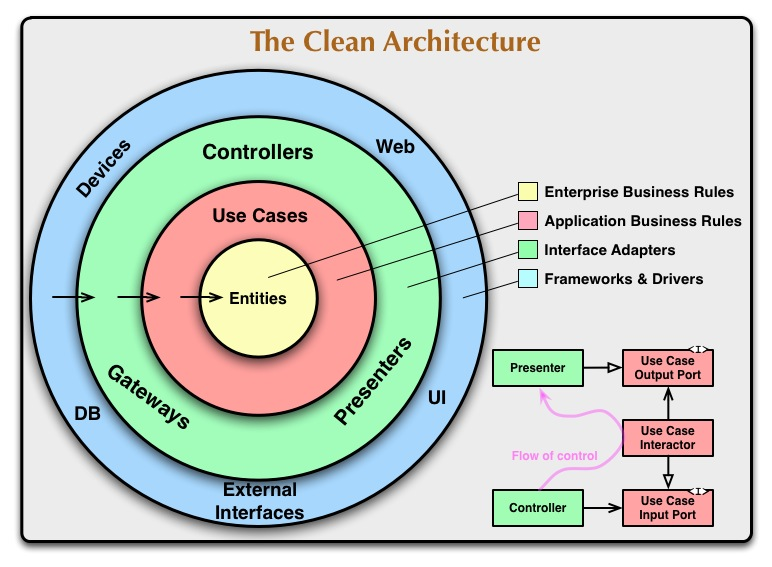
\includegraphics[width=0.7\textwidth]{../../resources/CleanArchitecture.jpeg}
	\caption{The Clean Architecture \cite{unclebob}}
	\label{fig:clean_arch}
\end{figure}

Figure \ref{fig:clean_arch} illustrates the clean architecture visually. Developing clean software 
architecture requires to comply with one important rule which is called the 
\textit{dependency rule}. The dependency rule states that any inner layer in the architecture may not 
depend on any outer layer while the opposite is possible and desired. To fulfill this rule, the most 
inner layer is called \textit{entities} and is to describe the most general or high-level business 
rules. Such rules are only business-dependent and have nothing to do with the rest of the developed 
software. Following this layer, comes the \textit{use cases}. Use cases define the same business rules 
on the application level which is to say, such implementation depends on the enterprise-wide business 
rules. \textit{Interface adapters} shown in the green circle are to serve as some sort of communication 
medium between the internal and external resources describing data format conversions. Finally, the 
most outer layer in the architecture is \textit{frameworks and adapters} which include third-party 
services such as databases, web frameworks, and so on. This layer contains the least amount of code 
development as well as a potential harm.

\paragraph{Diagrams.}
Figure \ref{fig:soft_arch} illustrates the UML class diagram with classes and relations between them. 
To get the top-down view, the most abstract or high-level classes are \textbf{ETL}, \textbf{ETLOperation} 
and \textbf{Data}. ETL may use zero or more ETLOperation and each such operation both consumes and 
produces OperationalData which is a subclass of the Data class. Each ETLOperation object is stored in 
the \textit{pipeline} attribute of an ETL object and the \textit{entity\_buffer} can be used for 
global data manipulations. It is the responsibility of the ETL object to keep track of termination 
condition(s) of the 
global program execution and not the ETLOperation objects. There are several private methods within 
the ETL to choose between the processing paradigms(i.e., sequential or parallel). A user of the 
library needs to create ETLOperation without directly interacting with it. In fact, ETLOperation is 
an abstract class with an unimplemented method \textit{run(\ldots)} as shown in the first row of table 
\ref{tab:abstract_methods} and for this purpose, there are three main subclasses of ETLOperation: 
\textbf{Extractor}, \textbf{Transformer} and \textbf{Loader}. All of these classes have also pure abstract 
methods \textit{extract(\ldots)}, \textit{transform(\ldots)} and \textit{load(\ldots)} respectively shown 
in the same table \ref{tab:abstract_methods}. This is to increase 
modularity, maintainability, and readability of the code by making sure that any ETLOperation is either of 
type Extractor or Transformer or Loader. One level down, there are also two classes that inherit from both 
the Extractor and Loader classes: \textbf{DatabaseOps} and \textbf{FileOps}. These two classes are used 
to abstract away two different extraction/loading paradigms(i.e., the ones that are local to the machine 
and the ones that need connectivity in the network). These operations can either be used for extraction or 
loading purposes with a single connection to a database or another machine and therefore, they inherit 
both the Extractor and Loader. The leaves of the class diagram contain the actual implementations of 
these methods and the user is able to initialize objects of these types.

\begin{figure}[H]
	\centering
	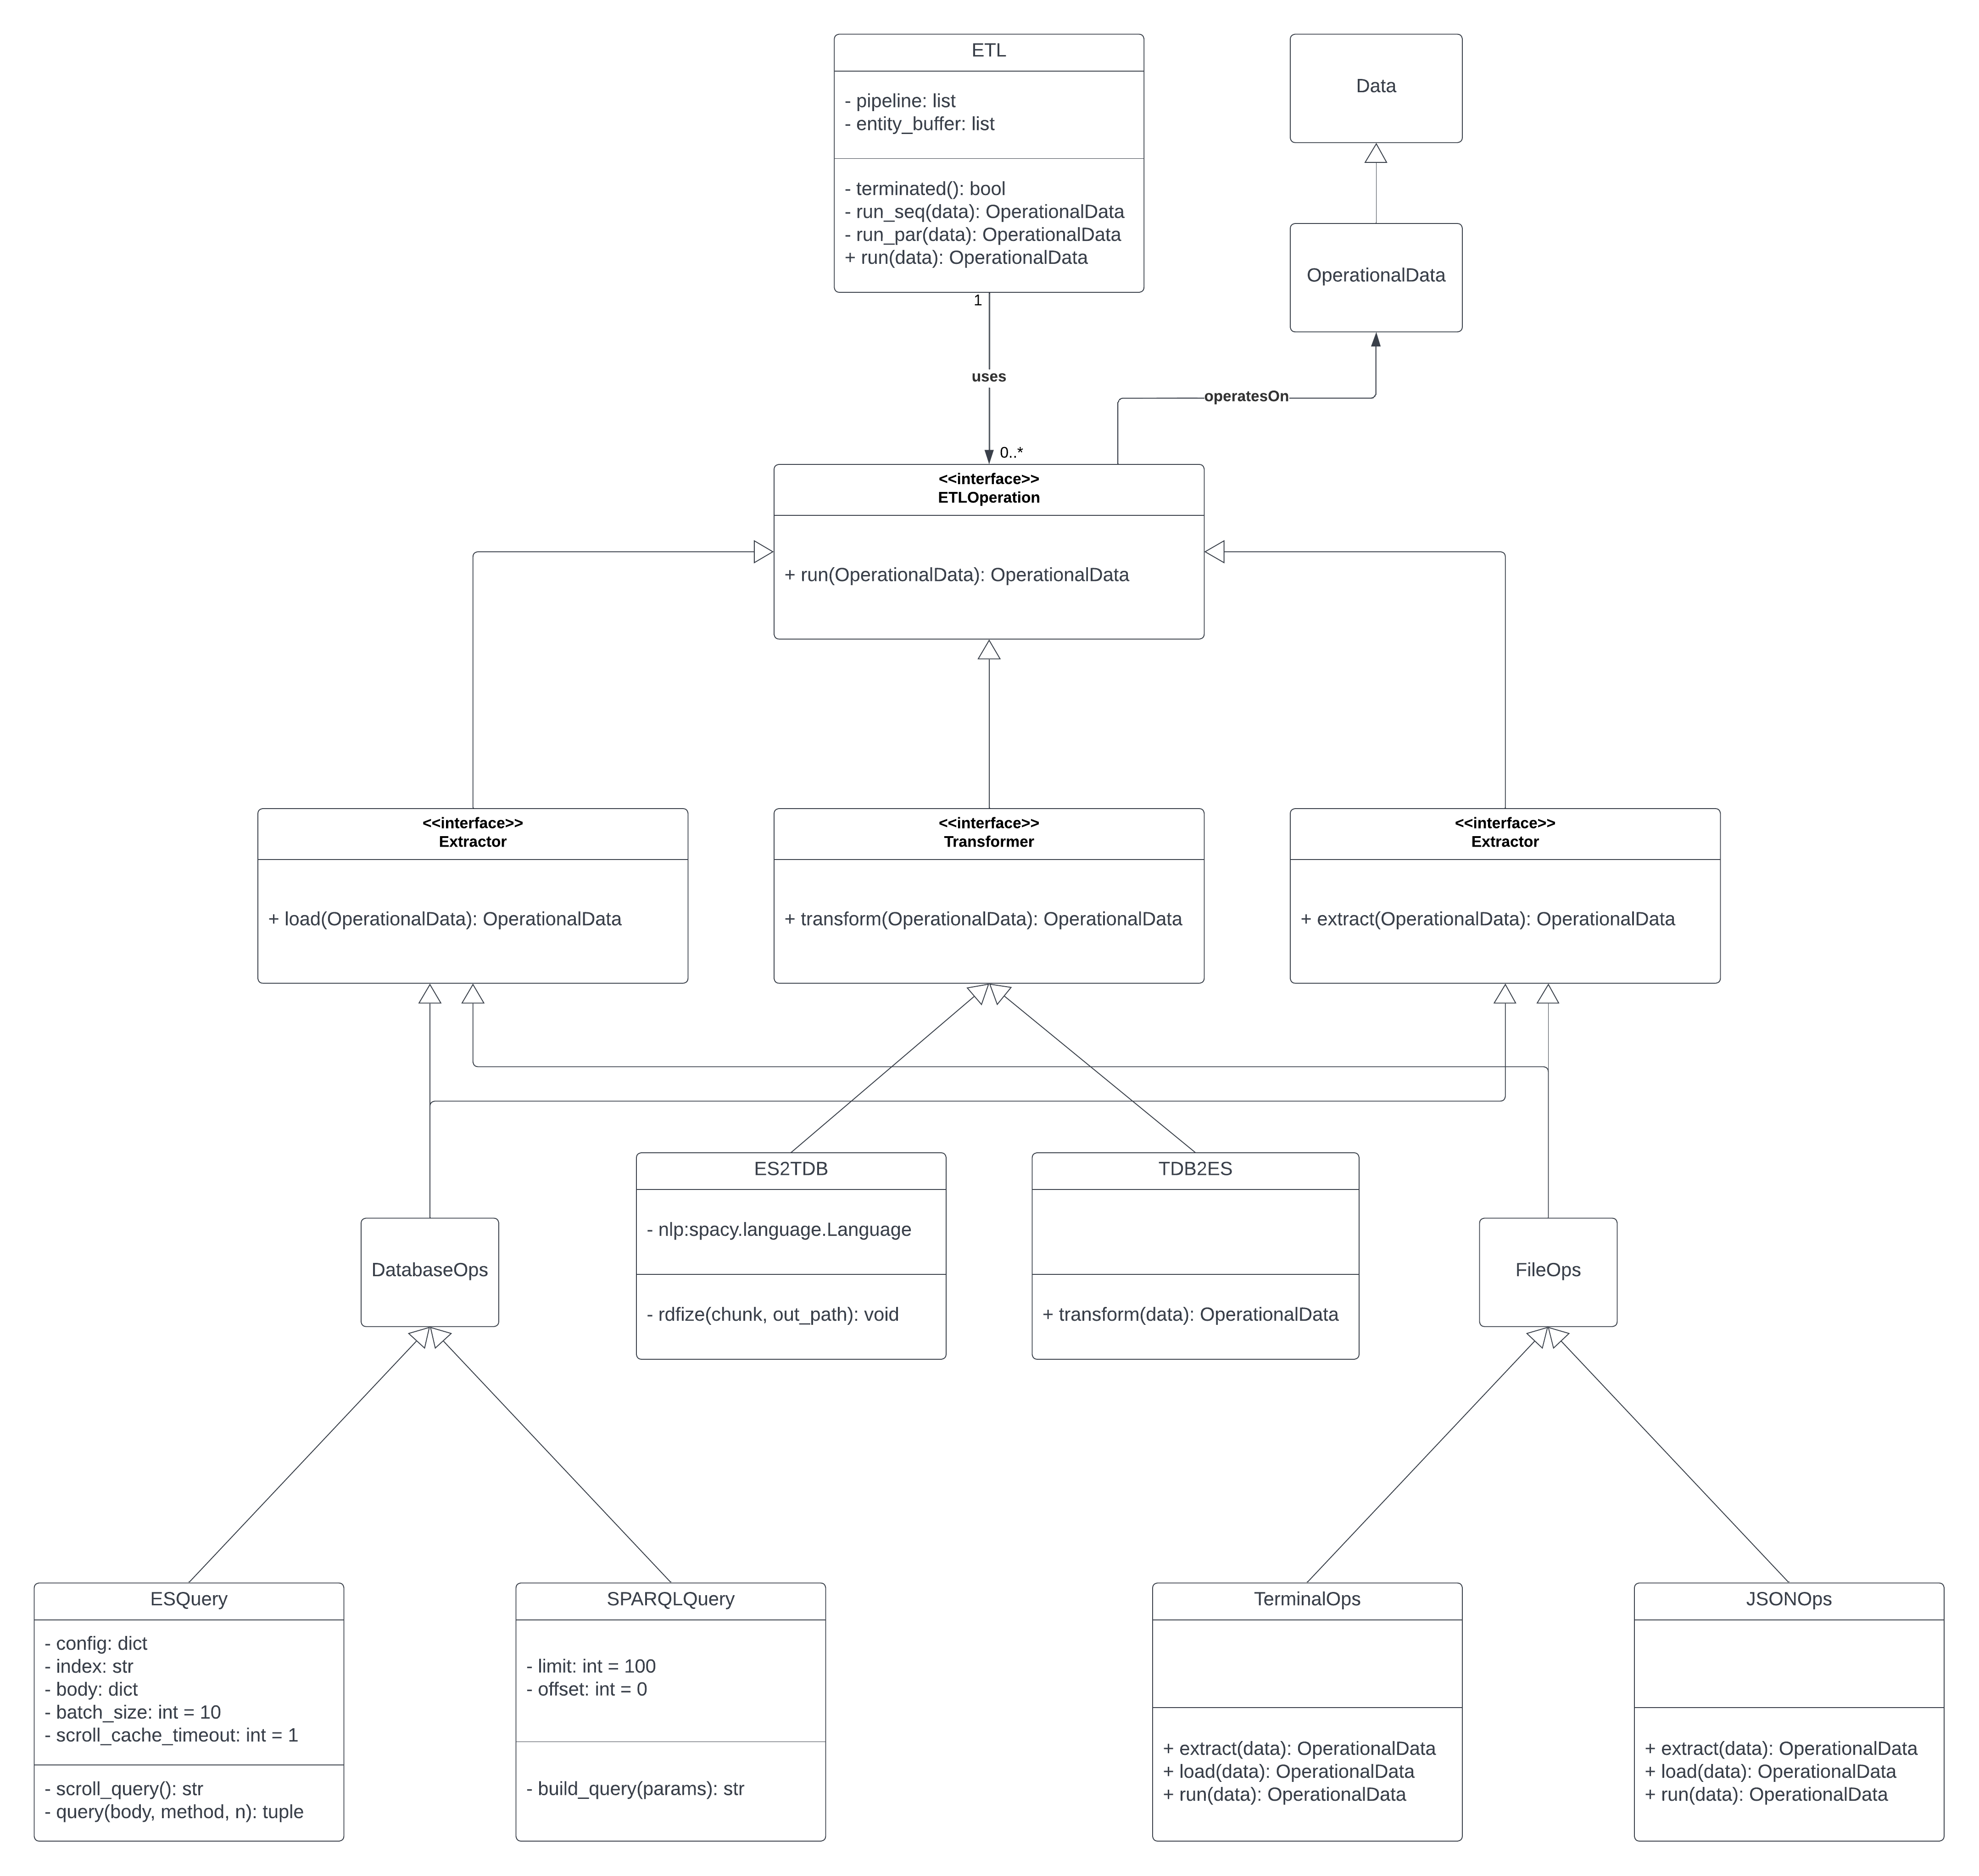
\includegraphics[width=0.95\textwidth]{../../resources/soft_arch.png}
	\caption{UML Class diagram}
	\label{fig:soft_arch}
\end{figure}

In case of any operational change in the business-logic level, one should be able to easily inherit his 
own \textit{implementation class}(i.e., the one which implements the abstract method(s) of its 
super/parent classes) from one or more of the top-level classes\footnote{The recommended classes to be 
inherited from are usually \textbf{DatabaseOps} and \textbf{FileOps} or \textbf{Transformer}.}. For 
example, if the database on which the KG is usually stored has to be changed to another database system, 
one can either modify the existing \textbf{SPARQLQuery} class or create a new, let's say, 
\textbf{MongoQuery} class inherited from Extractor and Loader. An instance of MongoQuery would be 
as easily 
usable as that of SPARQLQuery. This flexibility is due to the reason that this software architecture is 
very similar to and almost the same as the clean software architecture described previously; moving 
from the top of the hierarchy to the down is analogous to moving from the most inner circle to the 
most outer one in the clean software architecture.

\begin{table}[H]
	\centering
	\begin{tabular}{|c|c|}
		\hline
		\textbf{Class} & \textbf{Method} \\
		\hline
		ETLOperation & run(data: OperationalData) $\rightarrow$ OperationalData \\
		\hline
		Extractor & extract(data: OperationalData) $\rightarrow$ OperationalData \\
		\hline
		Transformer & transform(data: OperationalData) $\rightarrow$ OperationalData \\
		\hline
		Loader & load(data: OperationalData) $\rightarrow$ OperationalData \\
		\hline
	\end{tabular}
	\caption{Abstract methods}
	\label{tab:abstract_methods}
\end{table}

Users of this project are still the developers who are going to use \textit{knowledge acquisition} to 
make the resources semantically available for the final search engine processes. This being said, 
another type of user would be the end-users who are going to use/test the search engine by providing 
various textual queries and receiving the documents found and ranked by the search engine. Figure 
\ref{fig:soft_use_cases} demonstrate these use cases.

\begin{figure}[H]
\centering
\begin{subfigure}{.5\textwidth}
  \centering
  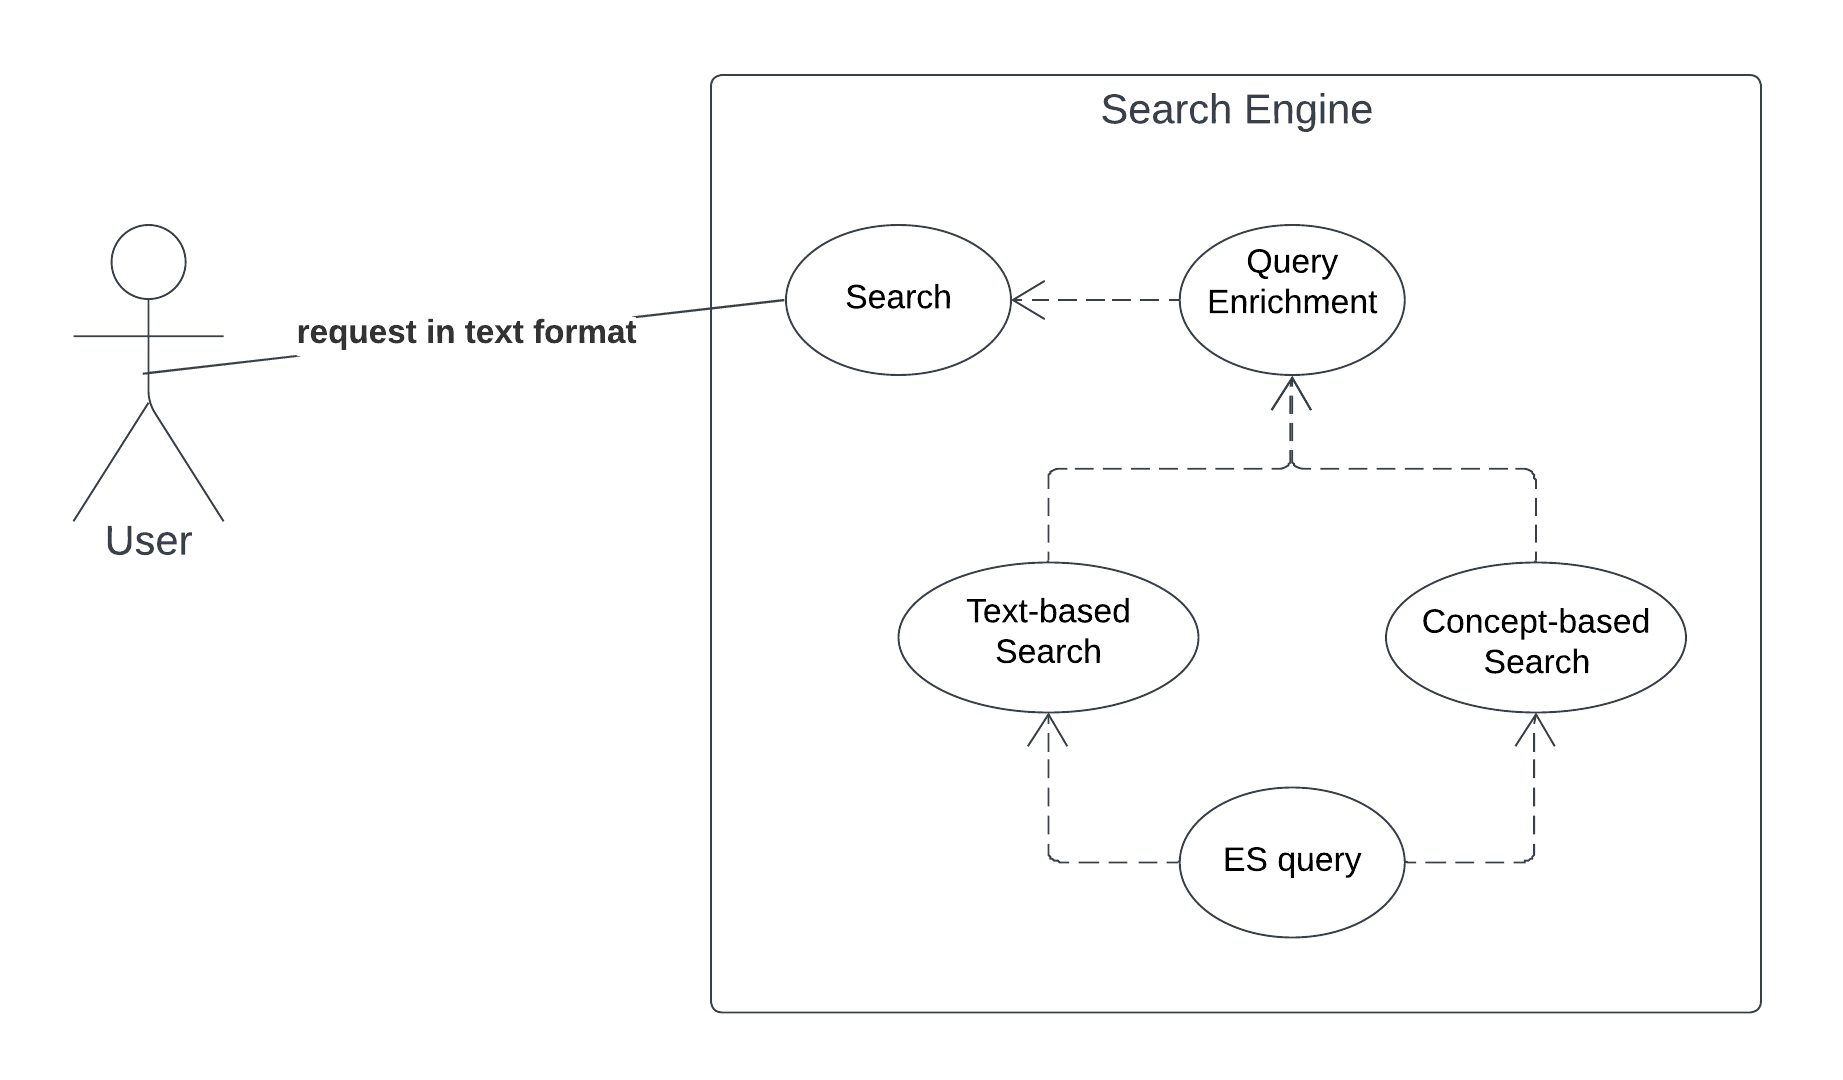
\includegraphics[width=.75\linewidth]{../resources/soft_use_case_1.png}
  \caption{Use case diagram for Knowledge Acquisition}
  \label{fig:subsoft_use_case_1}
\end{subfigure}%
\begin{subfigure}{.5\textwidth}
  \centering
  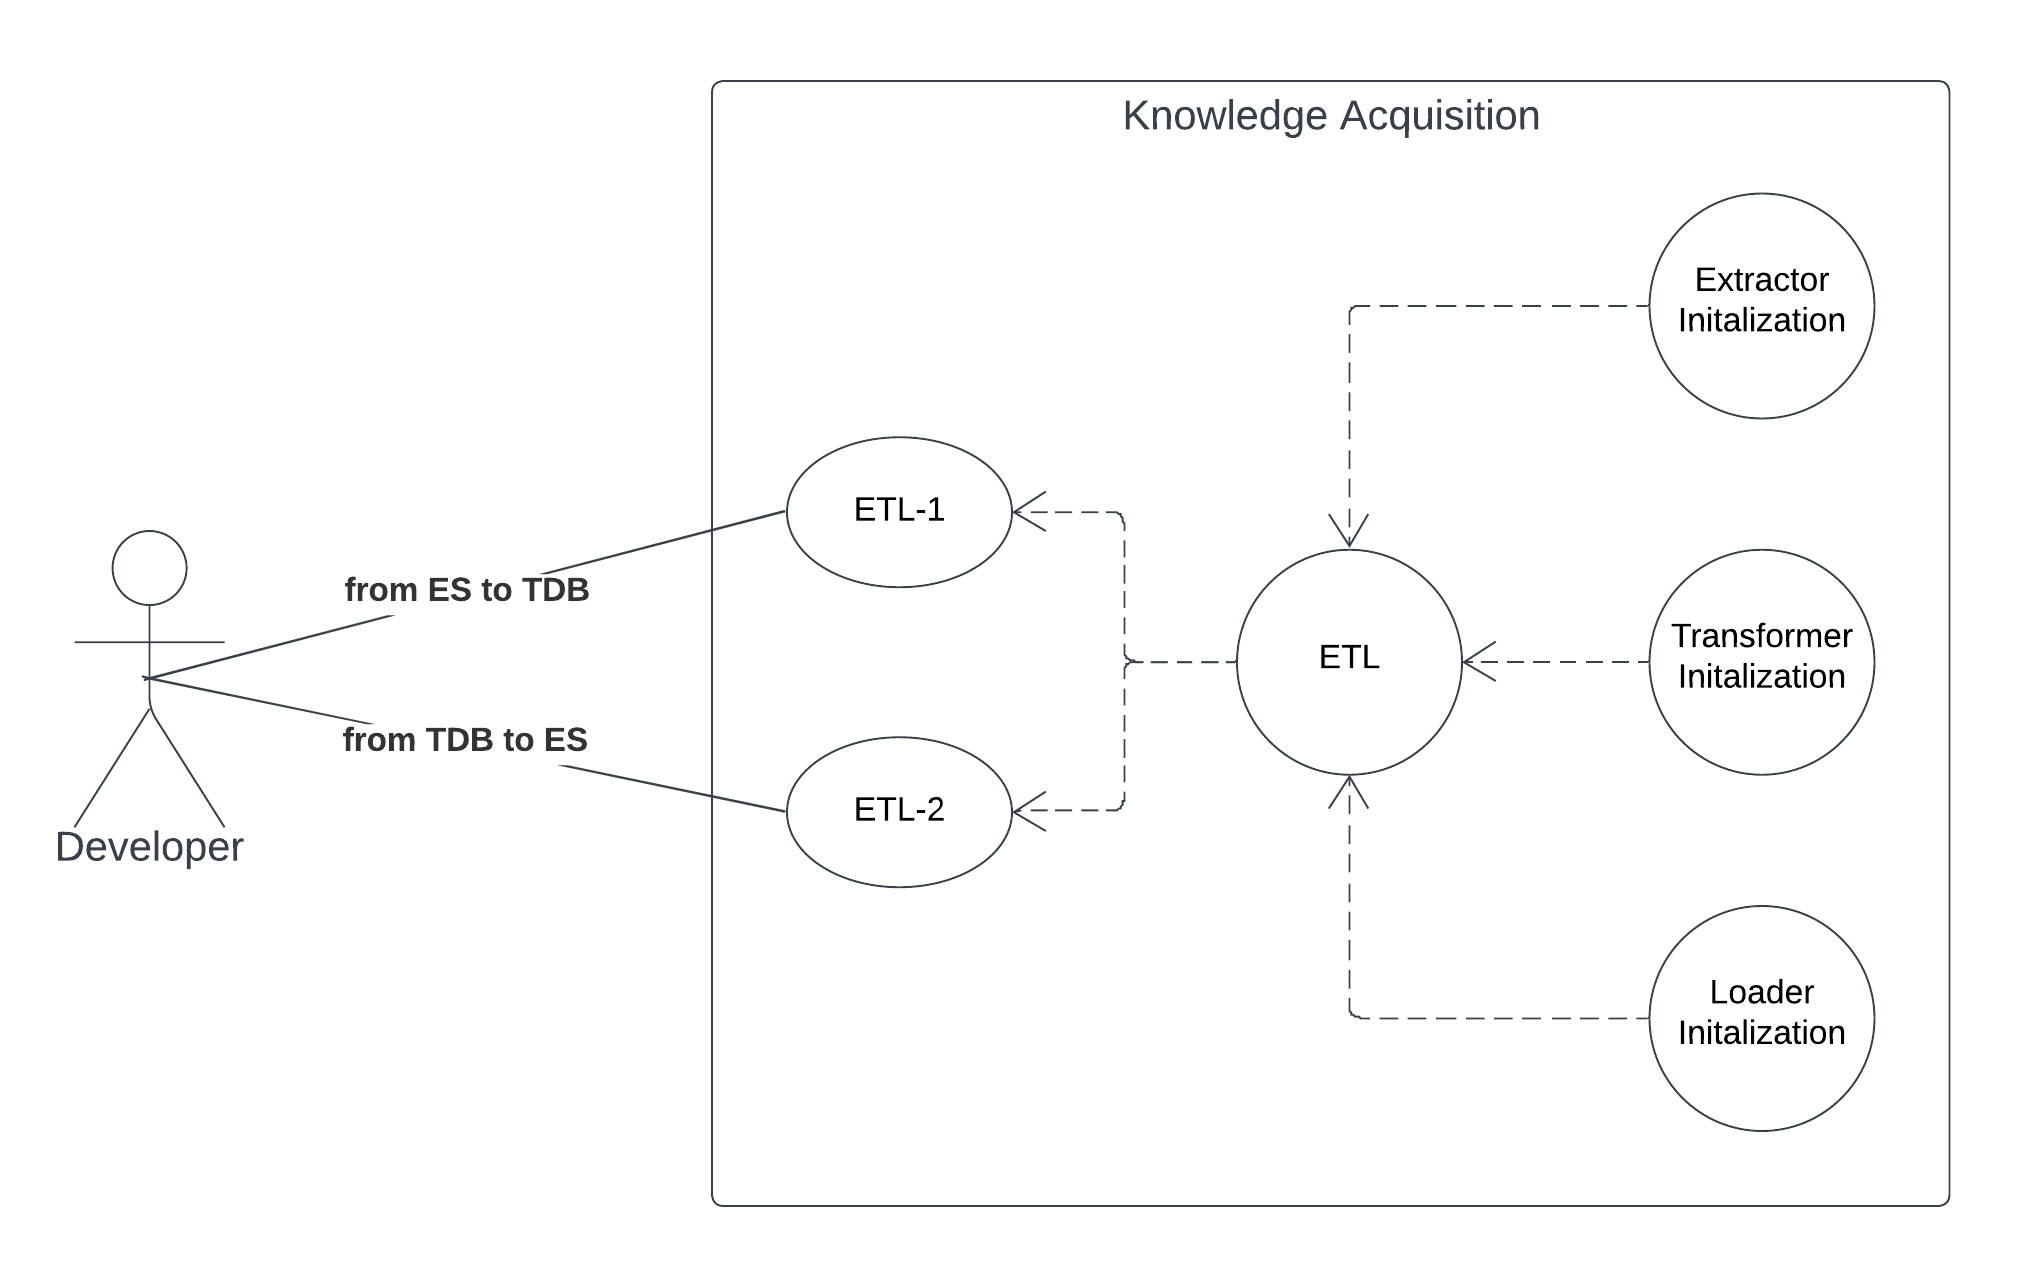
\includegraphics[width=.75\linewidth]{../resources/soft_use_case_2.png}
  \caption{Use case diagram for Search Engine}
  \label{fig:soft_use_case_2}
\end{subfigure}
\caption{Use case diagrams}
\label{fig:soft_use_cases}
\end{figure}

% Activity diagram is shown in tigure \ref{fig:soft_activity}.
% 
% \begin{figure}[H]
% 	\centering
% 	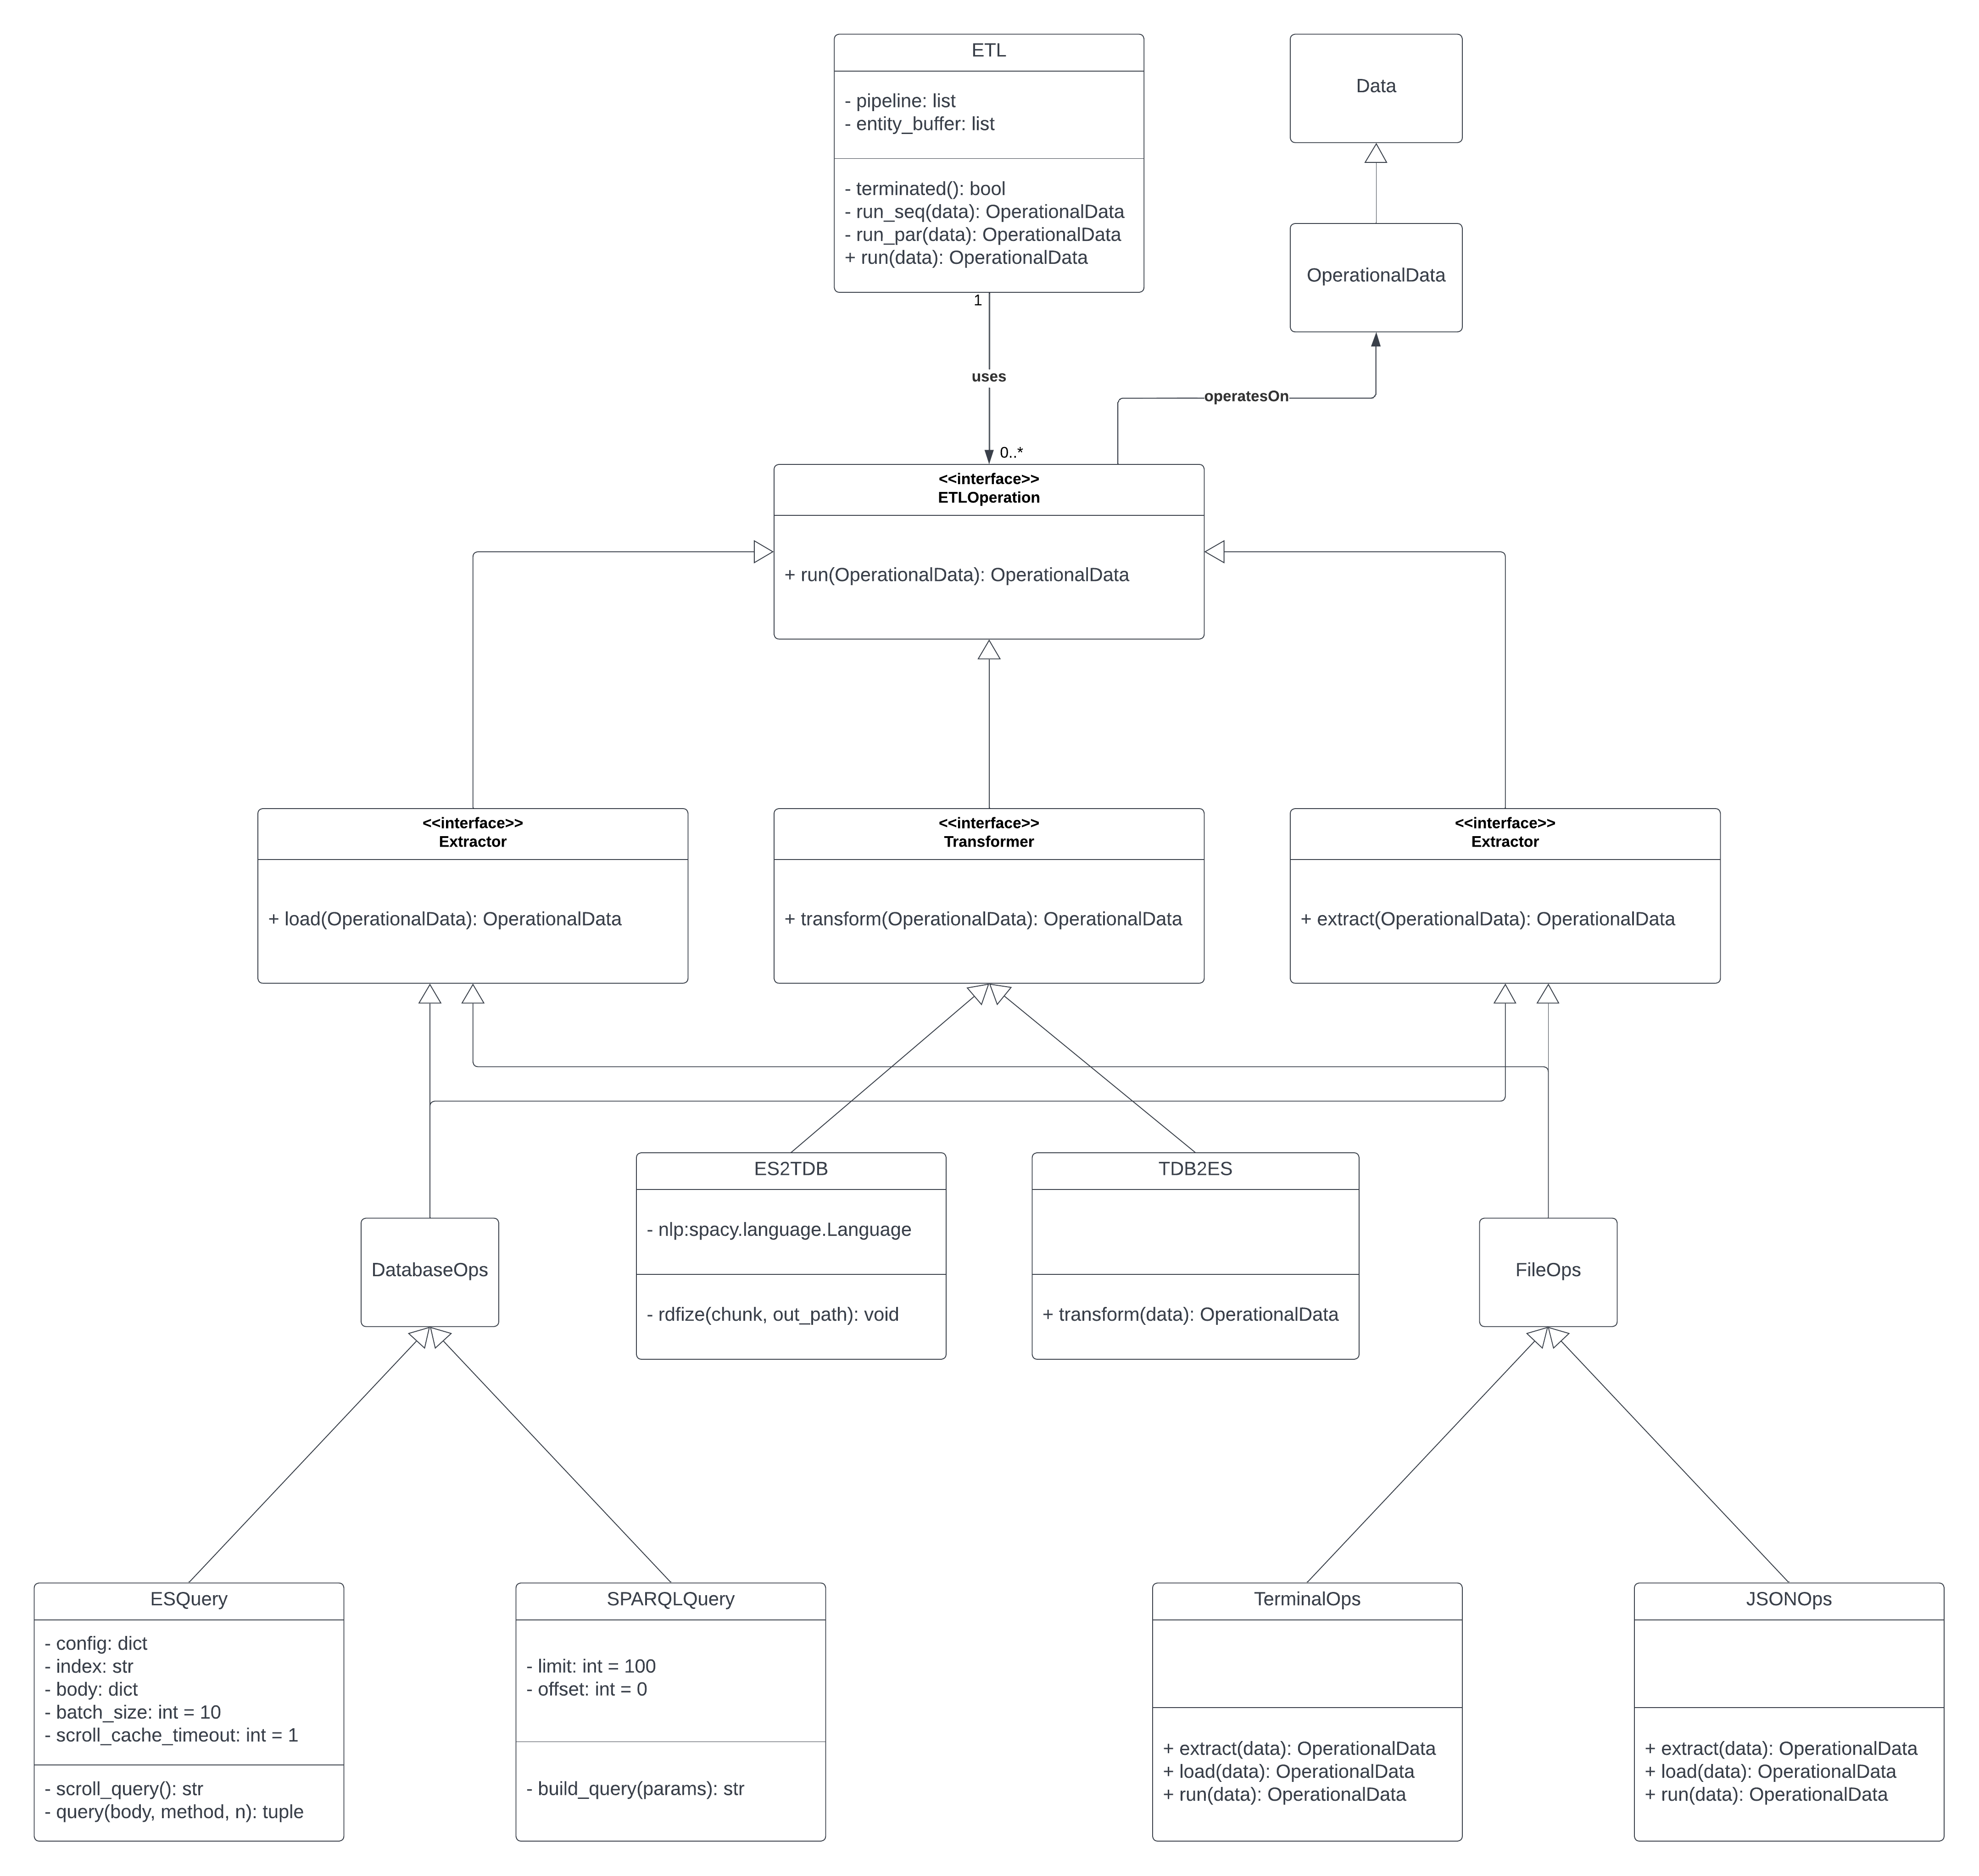
\includegraphics[width=0.75\textwidth]{../../resources/soft_arch.png}
% 	\caption{Activity diagram}
% 	\label{fig:soft_activity}
% \end{figure}

Interaction or sequence diagram is illustrated in figure \ref{fig:soft_sequence}. In order to 
perform ETL, three operations(i.e., Extractor, Transformer and Loader) are initialized. Extractor and 
Loader are usually required to create a session to be able to send requests to a database. An 
extractor 
object has an attribute called \textit{is\_active} which indicates if the most recent request was 
able to fetch some data. If nothing was fetched then this attribute is set to a boolean value of 
\textit{false}, otherwise, it is set to \textit{true}. The object of ETL class checks the value of 
\textit{is\_active} attribute of its first component(i.e., Extractor) in order to decide whether 
it should terminate or continue. If the termination criterion is not met then the residual 
components in the pipeline are executed.

\begin{figure}[H]
	\centering
	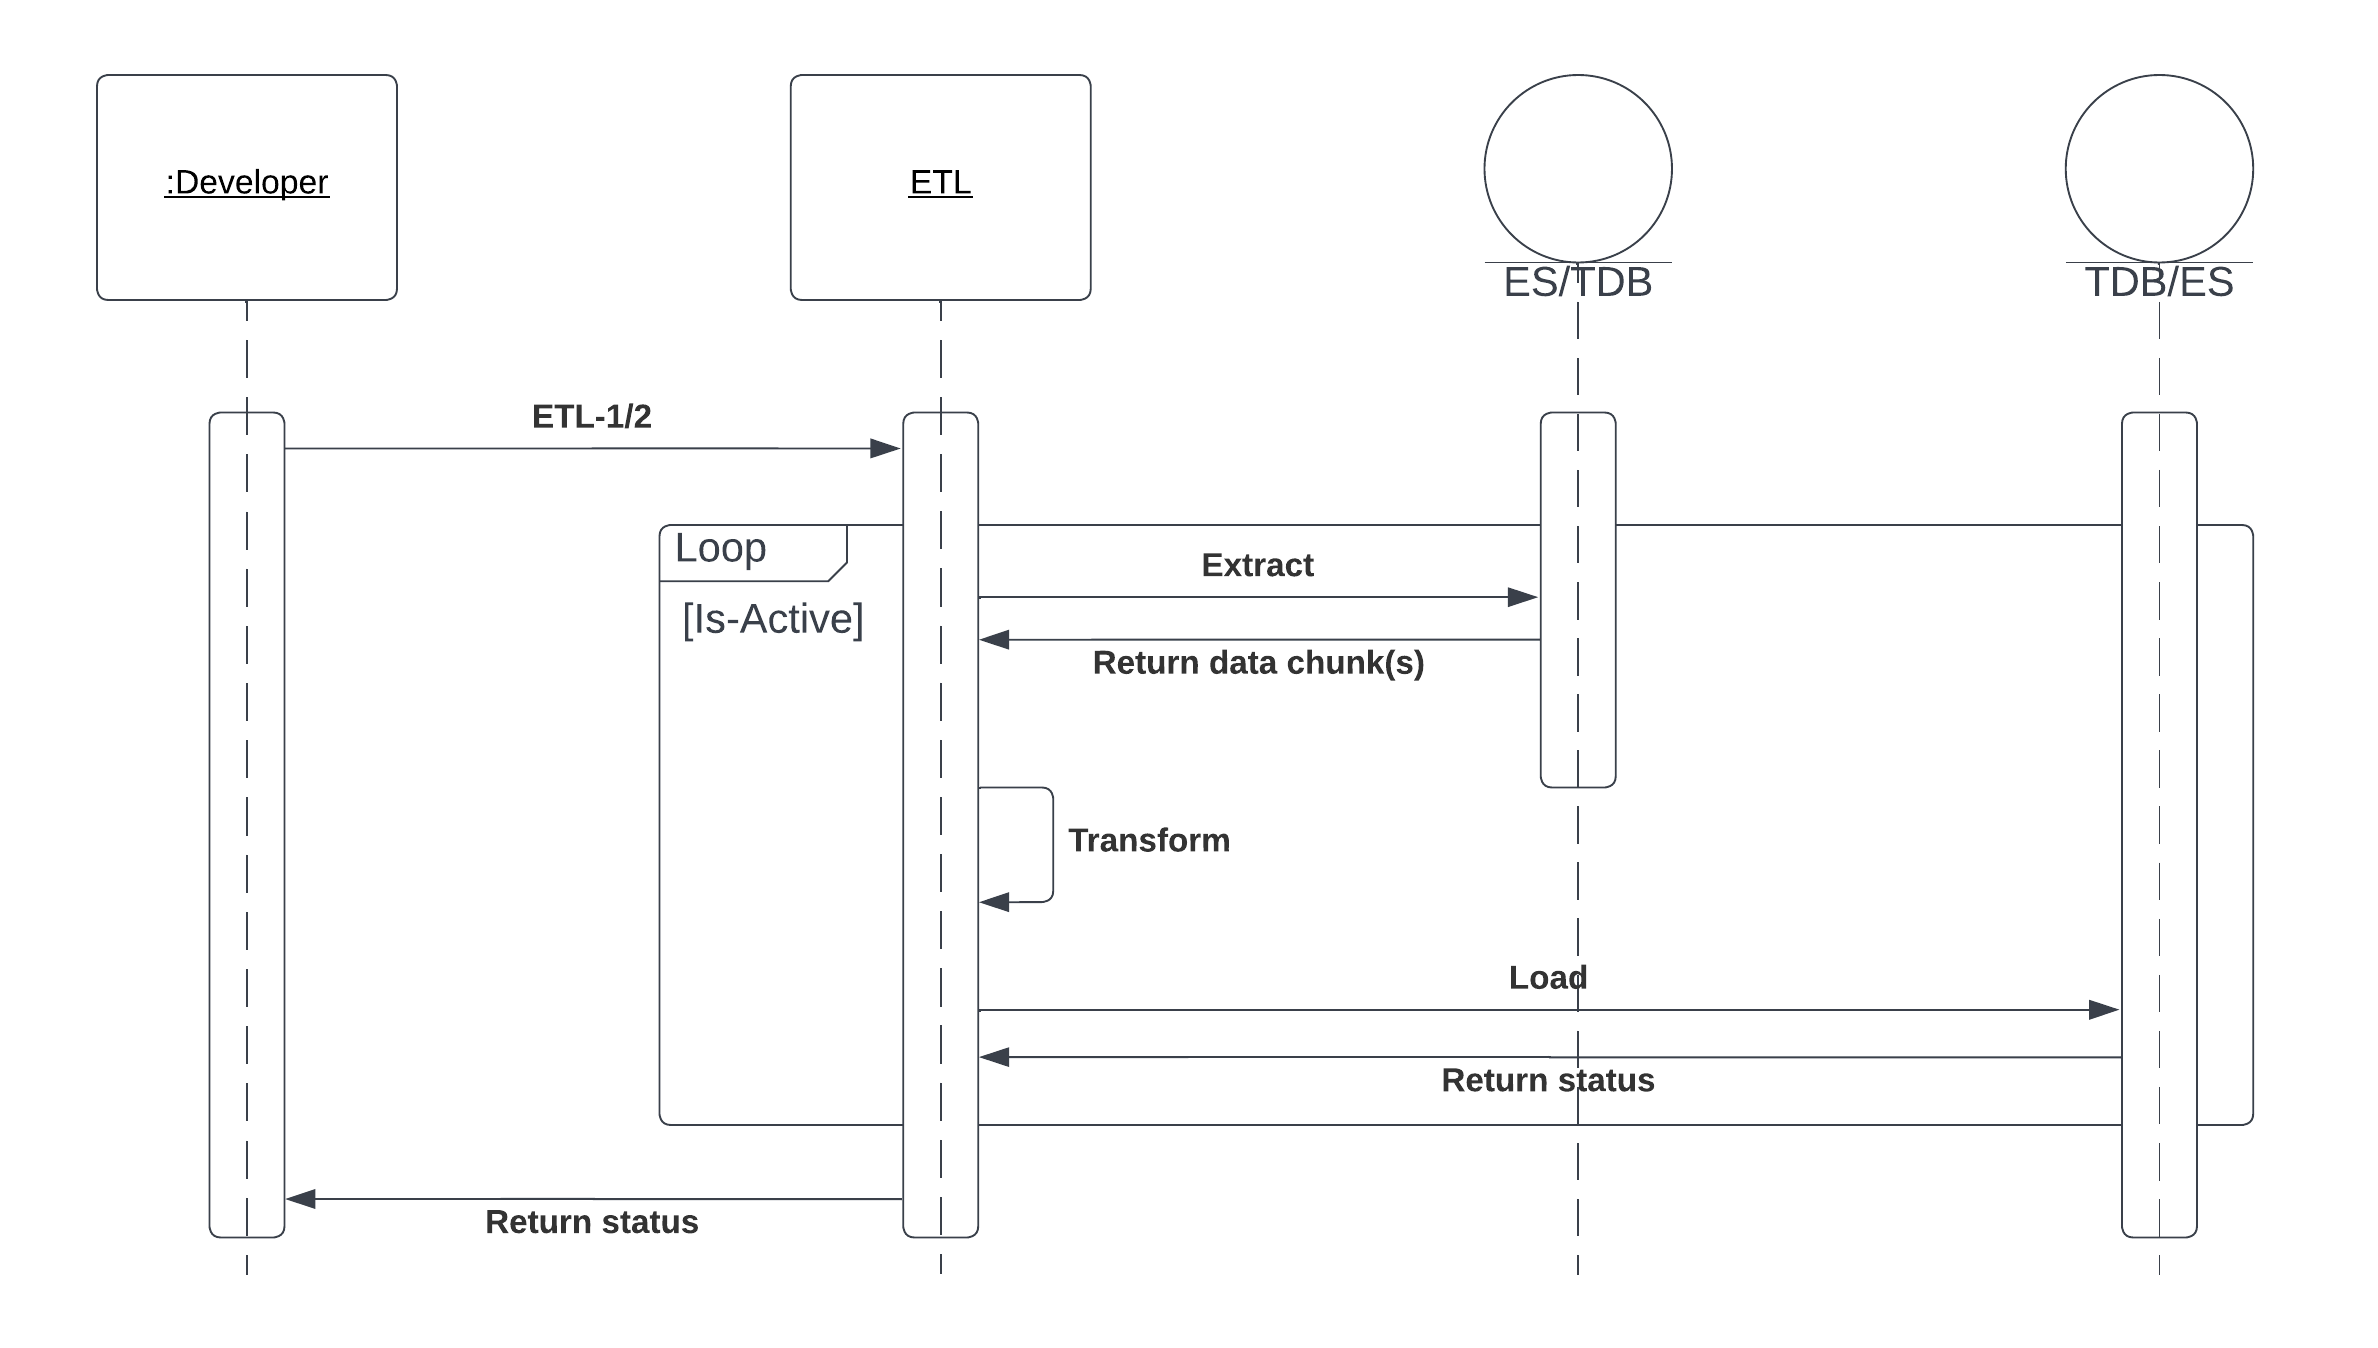
\includegraphics[width=0.95\textwidth]{../../resources/soft_sequence.png}
	\caption{Sequence diagram}
	\label{fig:soft_sequence}
\end{figure}

\paragraph{Sequential and Parallel Architecture.}
While developing the software to automate knowledge acquisition processes, we can also think of 
two main types of processing known as \textit{sequential} and \textit{parallel processing}. Writing 
a program in a sequential manner can be easy compared to the parallel one, however, there is a trade-off 
between the two. While sequentially running programs may usually be easier and faster to write, 
they may also become slower in execution time compared to that of parallel programs. Of course, this 
applies to programs that consists of many independent computations. The process of knowledge 
acquisition, in our case, contains many such computations as well. So, it is probably worth thinking 
about the software design from this aspect of processing too.
In addition to this, the real database of the company may contain millions, if not more, 
documents/products and to be able process all the database would potentially become intractable if 
executed sequentially. Parallelization with the right type of architecture and design could be 
very beneficial and improve the run-time quality several magnitudes of the order 10 or more depending 
on the machine specifications.

\begin{figure}[H]
	\centering
	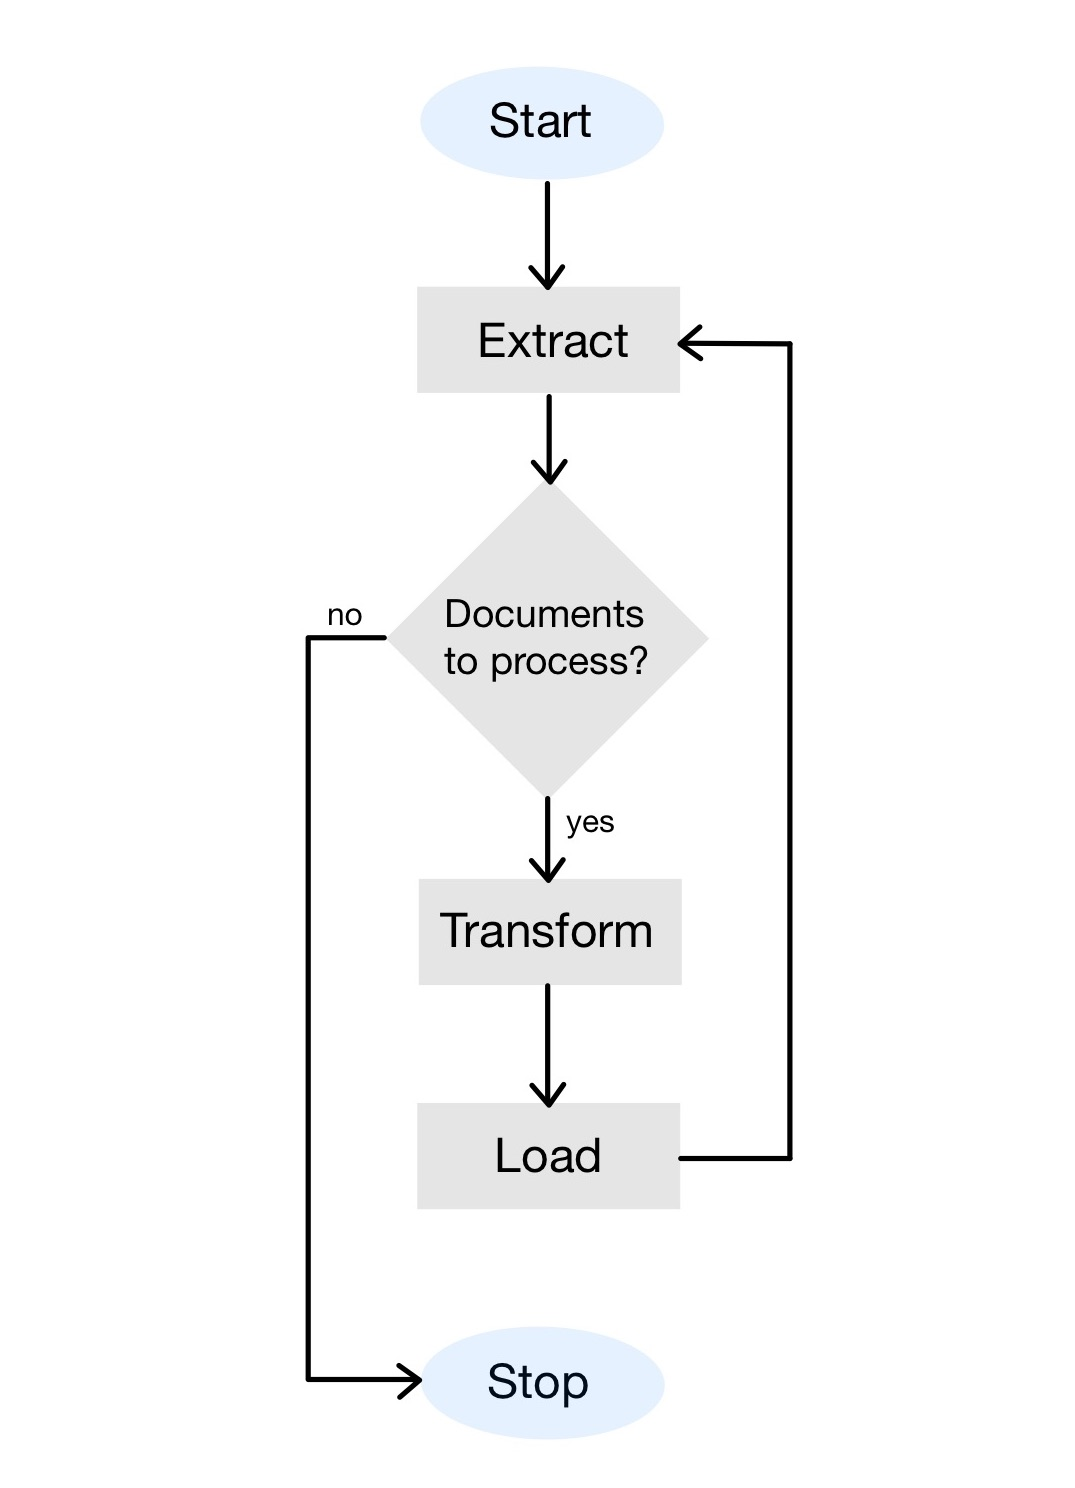
\includegraphics[width=0.55\textwidth]{../../resources/sequential_proc_arch.jpg}
	\caption{Sequential architecture}
	\label{fig:seq_arch}
\end{figure}

Figure \ref{fig:seq_arch} illustrate a simple sequential processing architecture that, by default, 
is selected when using the developed software. What this architecture tells us is that we run each 
subprocess (i.e., \textit{extract}, \textit{transform} and \textit{load}) once per a chunk of data or 
documents. Note that they may be invoked more than once within the scope of the whole process and 
this is due to the reason that the company's database may contain hundreds of GBs, if not thousands, 
all of which cannot be loaded at once to the local machine or any other ``regular'' computer that executes 
the program. For this reason, the documents or the data are extracted, transformed, and loaded in 
as many chunks as needed. If one iteration of ETL can only deal with 1000 documents and there are 
$10^9$ 
documents in the database, a million ETL processes are going to be executed one after another, in a 
sequential manner, in order to acquire 100\% of the knowledge completely.

\begin{figure}[H]
	\centering
	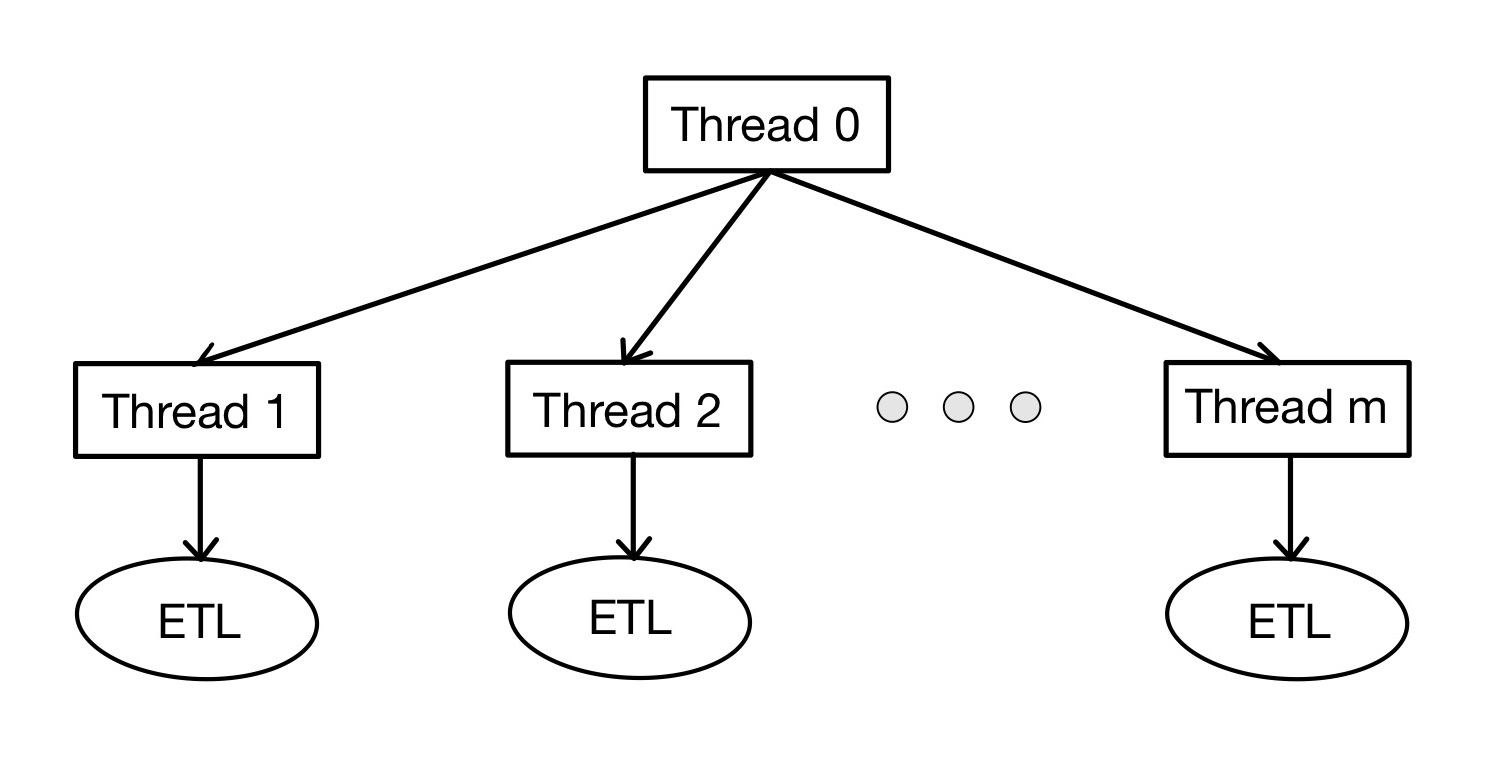
\includegraphics[width=0.75\textwidth]{../../resources/parallel_proc_arch.jpg}
	\caption{Parallel architecture}
	\label{fig:par_arch}
\end{figure}

In contrast to the sequential processing, it is also possible for one to separate ETL process to not 
wait for the other since they are completely independent. Realization of this simple fact leads us to 
develop a simple, yet faster-running, parallel processing architecture shown in figure 
\ref{fig:par_arch}.

\begin{figure}[H]
	\centering
	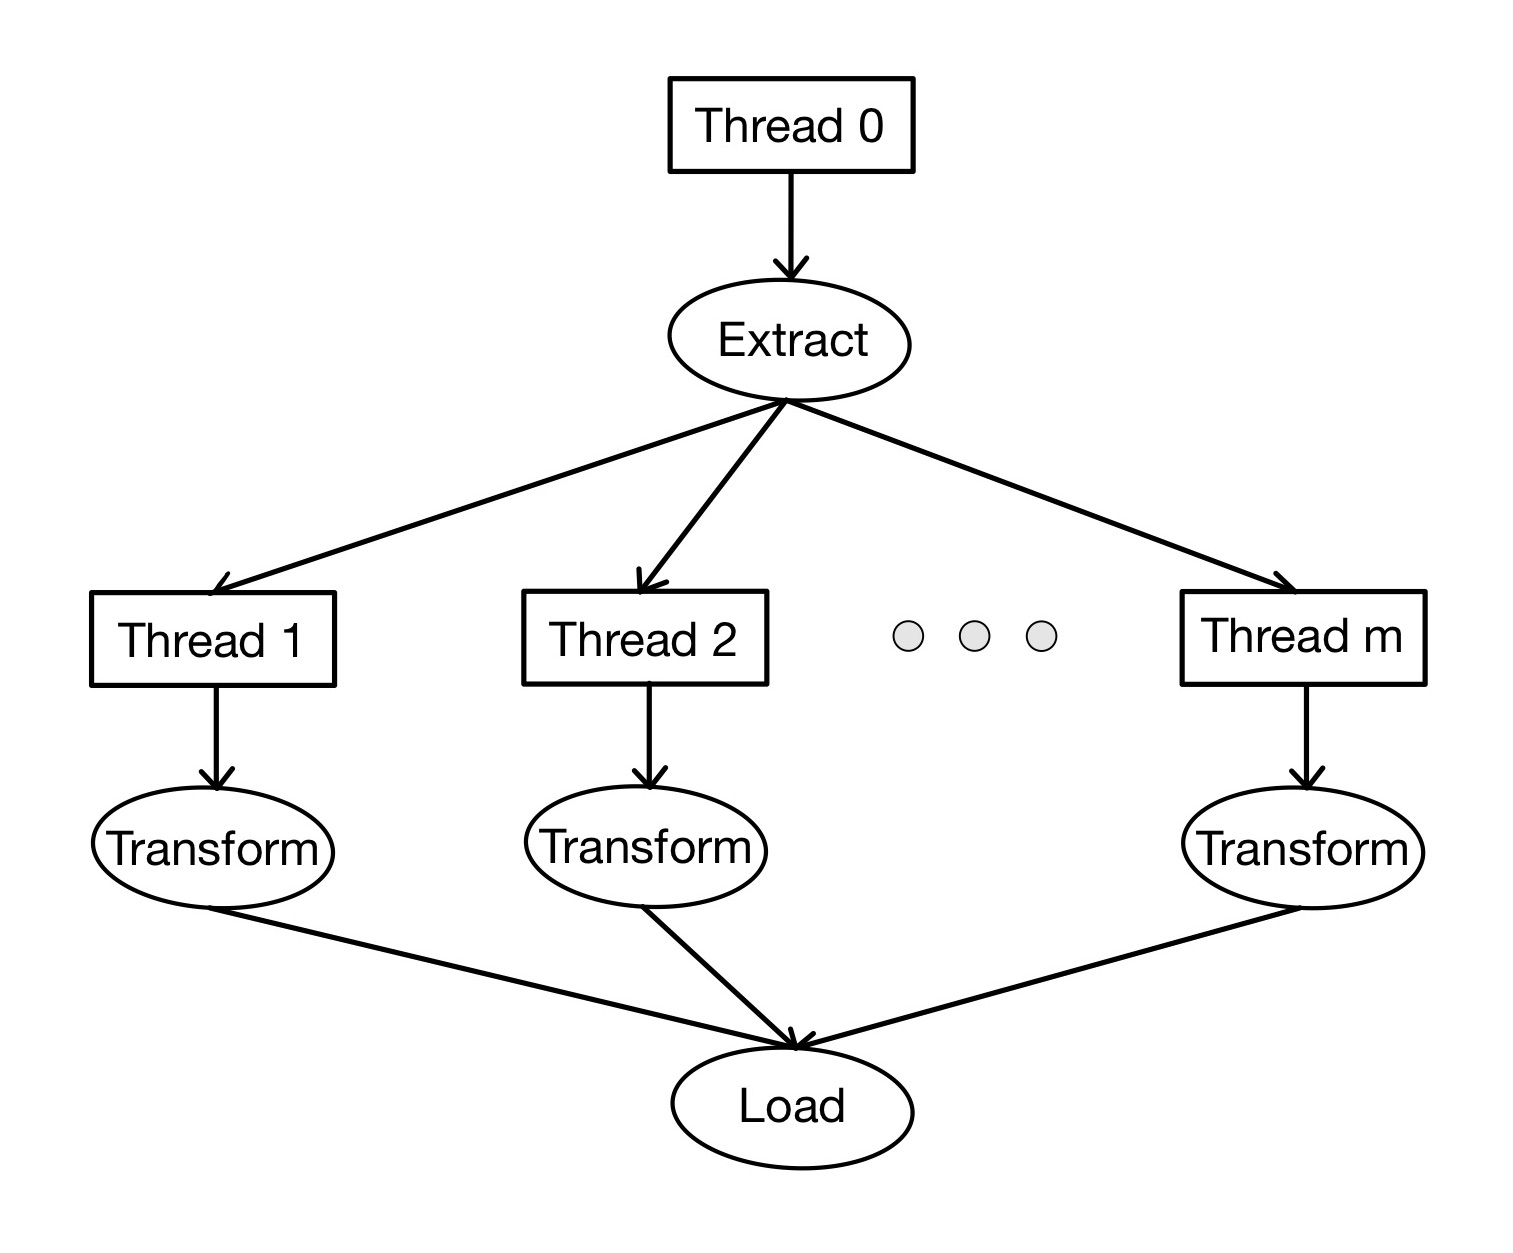
\includegraphics[width=0.75\textwidth]{../../resources/parallel_proc_arch2.jpg}
	\caption{Improved parallel architecture}
	\label{fig:par_arch2}
\end{figure}

Enhanced version of the architecture illustrated in figure \ref{fig:par_arch} can be easily realized 
if we excluded \textit{extract} and \textit{load} operations from running in a parallel fashion and 
only 
kept the \textit{transform} operation. The idea behind this architecture shown in figure 
\ref{fig:par_arch2} is the fact that each extraction and loading operation requires sending/receiving 
requests from/to a database running on some external network. It may be time-consuming to send and 
receive packets through the network when these operations are repeated many times. This is the reason, 
we can also improve the first parallel architecture by bringing the parallelism only to the 
\textit{transformation layer}. Therefore, instead of many extract-transform-load operations, we perform 
mass extraction then transformation of the vast amount of fetched documents in parallel, and finally, 
mass loading into another database.

\subsection{Specification and Implementation}

In this section, the developed software is described in terms of core implementational details that 
help to visualize and understand the underlying working principles of the carried operations. Mainly, 
there are several (sub)processes that have been described:

\begin{enumerate}
	\item Extract-Transform-Load pipeline execution
	\item Extraction process
	\item Transformation process
	\item Loading process
\end{enumerate}

The subprocesses(i.e., Extraction, Transformation and Loading) are first described in terms of 
their roles in the whole pipeline, and then the following sections break down these components by 
providing pseudo-codes and additional comments.

\paragraph{ETL Pipeline.}
\textit{ETL pipeline} is a sequence of \textbf{ETL Operations} that are executed in the given order. 
The existence of such a pipeline is for better modularity and readability. Components can easily be 
added, modified or removed from the pipeline. There are three ETL Operations or pipeline components 
that can be 
added to the ETL pipeline: \textit{Extractor}, \textit{Transformer} and \textit{Loader}. Figure 
\ref{fig:etl_pipeline} illustrates an example pipeline with these components and \textbf{*} sign on 
the top right side of each component indicates that there can be 0 or more such operations. The order 
of the components can also be arbitrary, however, it defines the processing order accordingly and 
therefore, depends on the use case of a user. Despite that, the common order of components in the 
pipeline is as shown below. Each operation takes in an input and returns an output of \textbf{Data} 
type. This constraint on the pipeline components is very helpful to build robustness and modularity.

\begin{figure}[H]
	\centering
	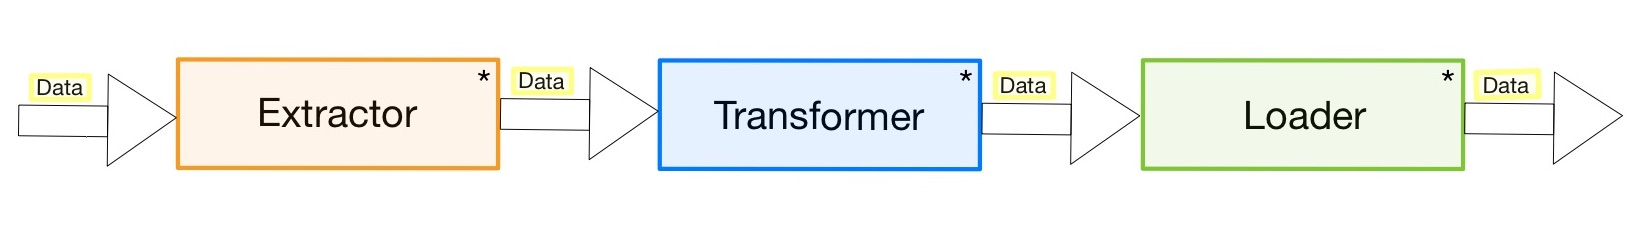
\includegraphics[width=\textwidth]{../../resources/etl_pipeline.jpg}
	\caption{ETL pipeline}
	\label{fig:etl_pipeline}
\end{figure}

The \textbf{Data} type is a simple class that has been created to serve as a unified data storage. 
By doing so, we can have restrictions, constraints and processes to check the validity of the data, 
if needed. Table \ref{tab:class_attr_data} shows the attributes and methods of this class.

\begin{table}[H]
	\centering
	\begin{tabular}{|p{0.5\textwidth}|p{0.5\textwidth}|}
		\hline
		\textbf{Attribute} & \textbf{Description} \\
		\hline
		data & Can be used to hold any type of data, however, the recommended format is the dictionary \\
		\hline
		\hline
		\textbf{Method} & \textbf{Description} \\
		\hline
		- & - \\
		\hline
	\end{tabular}
	\caption{Data Class Attributes/Methods}
	\label{tab:class_attr_data}
\end{table}

There are two different ETL pipelines used for the knowledge acquisition named as \textit{ETL-1} and 
\textit{ETL-2}. ETL-1 is to build and store a knowledge graph (KG) in a TDB database by fetching the raw 
documents from the original ES database. ETL-2 is to build a semantic ES (S-ES) database by using the 
already existing KG and make the documents searchable in a more semantic manner. For the detailed 
explaination of how the pipeline works, I am going to give demonstrative examples for both ETL pipelines 
and describe them step-by-step.

ETL-1 pipeline contains \textbf{ESQuery} as an \textit{extractor}, \textbf{ES2TDB} as a 
\textit{transformer} and \textbf{TerminalOps} as a \textit{loader}. The execution of this pipeline 
yields KG built upon the documents stored the original ES database. First, ESQuery 
fetches the documents chunk-by-chunk with the given document count per chunk and the total chunk count. 
Figure \ref{fig:es_doc_example} illustrates an example row of the ES database. Fetched documents are 
transformed by ES2TDB into OTTR instances as shown in figure \ref{fig:ottr_instance_example}.
This KG is then stored in a Jena's TDB database by the TerminalOps. Some of the final RDF/Turtle 
triples represented in the store KG are illustrated by figure \ref{fig:rdf_ttl_example} (see 
figure \ref{fig:rdf_ttl_example_full} for the full version). ETL-1 takes a relational ES database of 
the company as its input and builds a second Jena Fuseki (TDB) database which contains the KG.

% \begin{figure}[H]
% \centering
% \begin{subfigure}{\linewidth}
% 	\centering
% 
% 	\begin{table}[H]
% 		\begin{tabular}{|p{0.20\linewidth}|p{0.20\linewidth}|p{0.25\linewidth}|p{0.25\linewidth}|}
% 			\hline
% 			\textbf{PartFamily} & \textbf{PartNumber} & \textbf{PartFamilyName} & \textbf{PartNumberName} \\
% 			\hline
% 			90-22112018-056525 & LC1BL34U31 & [en] TeSys B contactor 4P 800A 240V AC - LC1BL34U31 & [en] TeSys B contactor 4P 800A 240V AC - LC1BL34U31 \\
% 			\hline
% 		\end{tabular}
% 	\end{table}
% 
% 	\caption{Document fetched from the ES database}
% 	\label{fig:es_doc_example}
% \end{subfigure}
% \end{figure}

% \begin{figure}[H]
% \ContinuedFloat
% 
% \begin{subfigure}{\textwidth}
%   \centering
% 
%   \begin{table}[H]
% 	  \begin{tabular}{|p{0.98\linewidth}|}
% 		  \hline
% 		  tp:createPartNumberInstance(tp:PNLC1BL34U31, tp:IDLC1BL34U31, tp:PF90-22112018-056525, tp:Text-6378022537900392513). \\
% 		  tp:createPartFamilyInstance(tp:PF90-22112018-056525, tp:ID90-22112018-056525, tp:Text-2992260873777870348). \\
% 		  tp:createTextInstance(tp:Text-6378022537900392513, "TeSys B contactor 4P 800A 240V AC"^^xsd:string, tp:Language-def, (tp:ID4P,tp:ID800A,tp:ID240V)). \\
% 		  tp:createTextInstance(tp:Text-2992260873777870348, "TeSys B contactor 4P 800A 240V AC - LC1BL34U31"^^xsd:string, tp:Language-def, (tp:ID4P,tp:ID800A,tp:ID240V,tp:IDLC1BL34U31)). \\
% 		  tp:createIdInstance(tp:IDLC1BL34U31, "LC1BL34U31"^^xsd:string). \\
% 		  tp:createIdInstance(tp:ID90-22112018-056525, "90-22112018-056525"^^xsd:string). \\
% 		  tp:createIdInstance(tp:ID4P, "4P"^^xsd:string). \\
% 		  tp:createIdInstance(tp:ID800A, "800A"^^xsd:string). \\
% 		  tp:createIdInstance(tp:ID240V, "240V"^^xsd:string). \\
% 		  \hline
% 	  \end{tabular}
%   \end{table}
% 
%   \caption{OTTR instance}
%   \label{fig:ottr_instance_example}
% \end{subfigure}
% \end{figure}

% \begin{figure}[H]
% \ContinuedFloat
% 
% \begin{subfigure}{\textwidth}
%   \centering
% 
%   \begin{table}[H]
% 	  \begin{tabular}{|p{0.31\linewidth}|p{0.31\linewidth}|p{0.31\linewidth}|}
% 		  \hline
% 		  \textbf{Subject} & \textbf{Predicate} & \textbf{Object} \\
% 		  \hline
% 		  \multirow{4}{*}{tp:PNLC1BL34U31} & rdf:type & tp:PartNumber \\
% 		   & gist:isIdentifiedBy & tp:IDLC1BL34U31 \\
% 		   & gist:isDescribedIn & tp:Text-6378022537900392513 \\
% 		   & tp:hasPartFamily & tp:PF90-22112018-056525 \\
% 		  \hline
% 		  \multirow{3}{*}{tp:PF90-22112018-056525} & rdf:type & tp:PartFamily \\
% 		   & gist:isIdentifiedBy & tp:ID90-22112018-056525 \\
% 		   & gist:isDescribedIn & tp:Text-2992260873777870348 \\
% 		  \hline
% 		  \multirow{3}{*}{tp:Text-6378022537900392513} & rdf:type & gist:Text \\
% 		   & gist:containedText & "TeSys B contactor 4P 800A 240V AC - LC1BL34U31" \\
% 		   & gist:isExpressedIn & tp:Language-def \\
% 		  \hline
% 		  \multirow{3}{*}{tp:IDLC1BL34U31} & rdf:type & gist:ID \\
% 		   & gist:uniqueText & "LC1BL34U31" \\
% 		   & gist:isPartOf & tp:Text-6378022537900392513 \\
% 		  \hline
% 	  \end{tabular}
%   \end{table}
% 
%   \caption{RDF/Turtle triples}
%   \label{fig:rdf_ttl_example}
% \end{subfigure}
% \caption{ETL from ES to TDB example}
% \label{fig:etl-1_example}
% \end{figure}

ETL-2 pipeline contains \textbf{SPARQLQuery} as an \textit{extractor}, \textbf{TDB2ES} as a 
\textit{transformer} and \textbf{JSONOps} as a \textit{loader}. This pipeline is executed after the 
execution of the first one and therefore, the existence of the KG as the single source of truth is 
already 
guaranteed. The necessary instances from the KG stored in the TDB database are fetched through one or 
more SPARQL queries as shown in figures \ref{fig:tdb_sparql_example} and 
\ref{fig:tdb_response_example}\footnote{tp = $<$https://ontologies.traceparts.com/$>$} 
\footnote{gist = $<$https://ontologies.semanticarts.com/gist/$>$} 
\footnote{rdf = $<$http://www.w3.org/1999/02/22-rdf-syntax-ns\#$>$}. Obtained responses are 
transformed to a suitable dictionary format according to the already-specified schema of the 
S-ES database. After the transformation of the fetched instances, the prepared Python dictionary 
is dumped to a JSON file as the result of the JSONOps execution. 
Figure \ref{fig:ses_json_example} illustrates the transformed version of the entities in a JSON format.
ETL-2 takes the KG stored in the Jena Fuseki (TDB) database as its input and builds a third ES 
database with some additional semantics.

\begin{figure}[H]
\centering
\begin{subfigure}{\linewidth}
	\centering

	\begin{table}[H]
		\begin{tabular}{|p{0.20\linewidth}|p{0.20\linewidth}|p{0.25\linewidth}|p{0.25\linewidth}|}
			\hline
			\textbf{PartFamily} & \textbf{PartNumber} & \textbf{PartFamilyName} & \textbf{PartNumberName} \\
			\hline
			90-22112018-056525 & LC1BL34U31 & [en] TeSys B contactor 4P 800A 240V AC - LC1BL34U31 & [en] TeSys B contactor 4P 800A 240V AC - LC1BL34U31 \\
			\hline
		\end{tabular}
	\end{table}

	\caption{Document fetched from the ES database}
	\label{fig:es_doc_example}
\end{subfigure}
\end{figure}

\begin{figure}[H]
\ContinuedFloat

\begin{subfigure}{\textwidth}
  \centering

  \begin{table}[H]
	  \begin{tabular}{|p{0.98\linewidth}|}
		  \hline
		  tp:createPartNumberInstance(tp:PNLC1BL34U31, tp:IDLC1BL34U31, tp:PF90-22112018-056525, tp:Text-6378022537900392513). \\
		  tp:createPartFamilyInstance(tp:PF90-22112018-056525, tp:ID90-22112018-056525, tp:Text-2992260873777870348). \\
		  tp:createTextInstance(tp:Text-6378022537900392513, "TeSys B contactor 4P 800A 240V AC"\^{}\^{}xsd:string, tp:Language-def, (tp:ID4P,tp:ID800A,tp:ID240V)). \\
		  tp:createTextInstance(tp:Text-2992260873777870348, "TeSys B contactor 4P 800A 240V AC - LC1BL34U31"\^{}\^{}xsd:string, tp:Language-def, (tp:ID4P,tp:ID800A,tp:ID240V,tp:IDLC1BL34U31)). \\
		  tp:createIdInstance(tp:IDLC1BL34U31, "LC1BL34U31"\^{}\^{}xsd:string). \\
		  tp:createIdInstance(tp:ID90-22112018-056525, "90-22112018-056525"\^{}\^{}xsd:string). \\
		  tp:createIdInstance(tp:ID4P, "4P"\^{}\^{}xsd:string). \\
		  tp:createIdInstance(tp:ID800A, "800A"\^{}\^{}xsd:string). \\
		  tp:createIdInstance(tp:ID240V, "240V"\^{}\^{}xsd:string). \\
		  \hline
	  \end{tabular}
  \end{table}

  \caption{OTTR instance}
  \label{fig:ottr_instance_example}
\end{subfigure}
% \end{figure}
% 
% \begin{figure}[H]
% \ContinuedFloat

\begin{subfigure}{\textwidth}
  \centering

  \begin{table}[H]
	  \begin{tabular}{|p{0.31\linewidth}|p{0.25\linewidth}|p{0.38\linewidth}|}
		  \hline
		  \textbf{Subject} & \textbf{Predicate} & \textbf{Object} \\
		  \hline
		  \multirow{4}{*}{tp:PNLC1BL34U31} & rdf:type & tp:PartNumber \\
		   & gist:isIdentifiedBy & tp:IDLC1BL34U31 \\
		   & gist:isDescribedIn & tp:Text-6378022537900392513 \\
		   & tp:hasPartFamily & tp:PF90-22112018-056525 \\
		  \hline
		  \multirow{3}{*}{tp:PF90-22112018-056525} & rdf:type & tp:PartFamily \\
		   & gist:isIdentifiedBy & tp:ID90-22112018-056525 \\
		   & gist:isDescribedIn & tp:Text-2992260873777870348 \\
		  \hline
		  \multirow{3}{*}{tp:Text-6378022537900392513} & rdf:type & gist:Text \\
		   & gist:containedText & "TeSys B contactor 4P 800A 240V AC - LC1BL34U31" \\
		   & gist:isExpressedIn & tp:Language-def \\
		  \hline
		  \multirow{3}{*}{tp:IDLC1BL34U31} & rdf:type & gist:ID \\
		   & gist:uniqueText & "LC1BL34U31" \\
		   & gist:isPartOf & tp:Text-6378022537900392513 \\
		  \hline
	  \end{tabular}
  \end{table}

  \caption{RDF/Turtle triples}
  \label{fig:rdf_ttl_example}
\end{subfigure}
\caption{ETL from ES to TDB example}
\label{fig:etl-1_example}
\end{figure}

\newpage
\begin{figure}[H]
\centering

\begin{subfigure}{\linewidth}
	\centering

	\begin{lstlisting}
	select ?subject ?predicate ?object
	where {
	  ?subject ?predicate ?object
	}
	limit 5
	offset 0
	\end{lstlisting}

	\caption{SPARQL query}
	\label{fig:tdb_sparql_example}
\end{subfigure}
% \end{figure}
% 
% \begin{figure}[H]
% \ContinuedFloat

\begin{subfigure}{\textwidth}
  \centering

  \begin{table}[H]
	  \begin{tabular}{|p{0.35\linewidth}|p{0.30\linewidth}|p{0.31\linewidth}|}
		  \hline
		  \textbf{Subject} & \textbf{Predicate} & \textbf{Object} \\
		  \hline
		  tp:ID10-12032019-066017 & rdf:type & gist:ID \\
		  tp:ID10-12032019-066017 & gist:uniqueText & "10-12032019-066017" \\
		  tp:IDZB5FA46C0 & rdf:type & gist:ID \\
		  tp:IDZB5FA46C0 & gist:uniqueText & "ZB5FA46C0" \\
		  tp:Text79763625448103550 & rdf:type & gist:Text \\
		  \hline
	  \end{tabular}
  \end{table}

  \caption{SPARQL response (KG)}
  \label{fig:tdb_response_example}
\end{subfigure}
\end{figure}

\begin{figure}[H]
\ContinuedFloat

\begin{subfigure}{\textwidth}
  \centering

  \begin{table}[H]
	  \begin{tabular}{|p{0.20\linewidth}|p{0.75\linewidth}|}
		  \hline
		  \textbf{Key} & \textbf{Value} \\
		  \hline
		  doc\_id & 90-22112018-056525:LC1BL34Q31 \\
		  \hline
		  uri & https://ontologies.traceparts.com/PF90-22112018-056525 \\
		  \hline
		  \multirow{4}{*}{concept\_uris} & tp:ID4P \\
		   & tp:IDLC1BL34Q31 \\
		   & tp:ID800A \\
		   & tp:ID240V \\
		  \hline
		  \multirow{2}{*}{searcable\_texts} & def: TeSys B contactor 4P 800A 240V AC - LC1BL34Q31 \\ 
		   & en: TeSys B contactor 4P 800A 240V AC - LC1BL34Q31 \\
		  \hline
	  \end{tabular}
  \end{table}

  \caption{RDF/Turtle triple}
  \label{fig:ses_json_example}
\end{subfigure}
\caption{ETL from TDB to ES example}
\label{fig:etl-2_example}
\end{figure}

\textit{ETL} algorithm shown in \ref{alg:etl} executes each pipeline component(i.e., extractor, 
transformer and loader) in the given order. If a user provides \{``parallelism'': 0\} in the data 
object to be given to \textit{run} method of the ETL object, the components are executed in a 
sequential fashion, one by one. Otherwise, the transformation operation is executed in a parallel 
fashion.

\begin{algorithm}[H]
\caption{ETL}\label{alg:etl}
\begin{algorithmic}
\Require \texttt{OperationalData}
\Ensure \texttt{OperationalData}

\While{\texttt{the process should not terminate}}
\If{\texttt{sequential run}}
	\For{\texttt{component in pipeline}}
		\State \texttt{data} = \texttt{component}.\texttt{run}(\texttt{data})
	\EndFor
\Else 	\Comment{for parallel run}
	\State \texttt{get extractor, transformer, loader from the pipeline}
	\State \texttt{extractor.run}(\texttt{data})
	\State \texttt{allocate $m$ buffers inside data object}
	\State \texttt{allocate $m$ threads to run transformer on the respective buffer}

	\For{\texttt{thread in threads}}
	\State \texttt{thread.run()}	\Comment{Each thread performs transformations on a subset of documents and stores the result temporarility on the corresponding index in buffer}
	\EndFor

	\State \texttt{wait for all $m$ threads to finish}
	\State \texttt{data} = \texttt{loader}.\texttt{run}(\texttt{data})
\EndIf
\EndWhile
\end{algorithmic}
\end{algorithm}

The \textit{pipeline} attribute of an ETL object can be initialized with an arbitrary number of 
ETL operations and in an arbitrary order. Such an arbitrary pipeline would work just fine if executed  
sequentially. Parallelized execution is only suitable for this project since there is only one of 
each operation per the whole ETL process. If the pipeline was to contain several extractors/loaders 
then a more generic implementation would be required to optimize it.

\paragraph{Extractor.}
The Extractor class is a process-only class\footnote{By process-only class, I mean a class that 
consists of only methods and not attributes since the whole purpose of using them is mostly 
processing the given data and returning the modified version of it back.}. Table 
\ref{tab:class_attr_extractor} shows the attributes and methods of the Extractor class. There are 
no attributes and only two abstract methods one of which(i.e., \texttt{run(\ldots)}) is inheretied 
from the parent class ETLOperation.

\begin{table}[H]
	\centering
	\begin{tabular}{|p{0.5\textwidth}|p{0.5\textwidth}|}
		\hline
		\textbf{Attribute} & \textbf{Description} \\ 
		- & - \\
		\hline
		\hline
		\textbf{Method} & \textbf{Description} \\ 
		\hline
		extract(data: OperationalData) $\rightarrow$ OperationalData & abstract \\
		\hline
		run(data: OperationalData) $\rightarrow$ OperationalData & abstract, inherited \\
		\hline
	\end{tabular}
	\caption{Extractor Class Attributes/Methods}
	\label{tab:class_attr_extractor}
\end{table}

\begin{algorithm}
\caption{ESQuery/SPARQLQuery-Extractor}\label{alg:etl_extractor}
\begin{algorithmic}
\Require requestBody, method, url, numChunk
\Ensure docs (as a list of numChunk chunks)

\State session = createSession()	\Comment{created once within an object}
\If{scrollRequest}	\Comment{getting response partially}
	\State requestBody = buildScrollQuery()	\Comment{different implementation for different databases}
\EndIf
% \algstore{myalgextractor}
% \end{algorithmic}
% \end{algorithm}
% 
% \begin{algorithm}
% \begin{algorithmic}
% \algrestore{myalgextractor}
\State response = session.request(requestBody, method, url)
\State extract \textbf{header} and \textbf{hits} from \textbf{response}
\State chunks = []	\Comment{initialize chunks as an empty list}
\State chunkSize = len(hits) / numChunk

\For{$i$ in $\{0, \cdots, \text{numChunk}-1\}$}
	\State chunks.append(hits[$i*\text{chunkSize}$ : $(i+1)*\text{chunkSize}$)	\Comment{add sublist of documents}
\EndFor
\State chunks.append(hits[$(\text{numChunk}-1)*\text{chunkSize}$ : ])	\Comment{add the residual documents, if any}

\State \Return header, chunks
\end{algorithmic}
\end{algorithm}

% \begin{algorithm}[H]
% \caption{ESQuery/SPARQLQuery-Extractor}\label{alg:etl_extractor}
% \begin{algorithmic}
% \Require requestBody, method, url, numChunk
% \Ensure docs (as a list of numChunk chunks)
% 
% \State session = createSession()	\Comment{created once within an object}
% \If{scrollRequest}	\Comment{getting response partially}
% 	\State requestBody = buildScrollQuery()	\Comment{different implementation for different databases}
% \EndIf
% 
% \State response = session.request(requestBody, method, url)
% \State extract \textbf{header} and \textbf{hits} from \textbf{response}
% \State chunks = []	\Comment{initialize chunks as an empty list}
% \State chunkSize = len(hits) / numChunk
% 
% \For{$i$ in $\{0, \cdots, \text{numChunk}-1\}$}
% 	\State chunks.append(hits[$i*\text{chunkSize}$ : $(i+1)*\text{chunkSize}$)	\Comment{add sublist of documents}
% \EndFor
% \State chunks.append(hits[$(\text{numChunk}-1)*\text{chunkSize}$ : ])	\Comment{add the residual documents, if any}
% 
% \State \Return header, chunks
% \end{algorithmic}
% \end{algorithm}

Algorithm \ref{alg:etl_extractor} illustrates how the specific extraction processes from ElasticSearch 
(ESQuery) and TDB(SPARQLQuery) are performed. The only important difference between these processes is 
in the query-building part. Scroll queries are known as queries performed on the databases resulting 
in 
partial responses. When the response may be too huge in size, we request only a part of it iteratively 
until we reach to the end of it and this is the main reason why scroll queries are very useful. More 
specifically, the scroll queries for the request body are built differently for ES and TDB endpoints. For 
example, building a scroll query requires a \textit{scroll ID} of the last query in the ES database while there 
is an offset value set by the user to get the next piece of partial response in the TDB database. 
So, the implementation of building scroll queries has solely built upon scroll IDs and offset values 
for the respective endpoints.

\paragraph{Transformer.}
Transformer is a pure abstract class which is used to define an interface for different 
transformation implementations. Table \ref{tab:class_attr_transformer} illustrates the 
attributes and methods of this class.

\begin{table}[H]
	\centering
	\begin{tabular}{|p{0.5\textwidth}|p{0.5\textwidth}|}
		\hline
		\textbf{Attribute} & \textbf{Description} \\ 
		nlp & spacy.language.Language \\
		\hline
		\hline
		\textbf{Method} & \textbf{Description} \\ 
		\hline
		transform(data: OperationalData) $\rightarrow$ OperationalData & abstract \\
		\hline
		run(data: OperationalData) $\rightarrow$ OperationalData & abstract, inherited \\
		\hline
	\end{tabular}
	\caption{Transformer Class Attributes/Methods}
	\label{tab:class_attr_transformer}
\end{table}

Algorithms \ref{alg:etl_transformer_es2tdb} and \ref{alg:etl_transformer_tdb2es} illustrate how 
the specific transformation processes are executed to transform entites coming from ES(original 
database) to TDB(knowledge graph storage) and from TDB(knowledge graph storage) to ES(semantic ES 
database) respectively.

\begin{algorithm}
\caption{ES2TDB-Transformer}\label{alg:etl_transformer_es2tdb}
\begin{algorithmic}
\Require docs
\Ensure rdf/ttl file

\State file = open(filepath)
\For{doc in docs}
	\State fetch \textbf{pfID} from \textbf{doc}
	\State fetch \textbf{pnNumber} from \textbf{doc}
	\State fetch \textbf{pfNamesDict} from \textbf{doc}
	\State fetch \textbf{pnNamesDict} from \textbf{doc}

	\State file.write(processID(pfID))	\Comment{processID returns ID intialization string in OTTR format}
	\State file.write(processID(pnNumber))
\algstore{myalges2tdb}
\end{algorithmic}
\end{algorithm}

\begin{algorithm}
\begin{algorithmic}
\algrestore{myalges2tdb}
	\For{language, pfName in pfNamesDict}
	\State file.write(processPF(nlp, pfID, pfName, language)	\Comment{processPF returns PartFamily initialization string in OTTR format}
	\EndFor

	\For{language, pfName in pnNamesDict}
	\State file.write(processPN(nlp, pnNumber, pnName, language) 	\Comment{processPN returns PartNumber initialization string in OTTR format}
	\EndFor
\EndFor

\State compileOTTR(filepath)	\Comment{compilation of generated OTTR instance file(s)}
\end{algorithmic}
\end{algorithm}

% \begin{algorithm}[H]
% \caption{ES2TDB-Transformer}\label{alg:etl_transformer_es2tdb}
% \begin{algorithmic}
% \Require docs
% \Ensure rdf/ttl file
% 
% \State file = open(filepath)
% \For{doc in docs}
% 	\State fetch \textbf{pfID} from \textbf{doc}
% 	\State fetch \textbf{pnNumber} from \textbf{doc}
% 	\State fetch \textbf{pfNamesDict} from \textbf{doc}
% 	\State fetch \textbf{pnNamesDict} from \textbf{doc}
% 
% 	\State file.write(processID(pfID))	\Comment{processID returns ID intialization string in OTTR format}
% 	\State file.write(processID(pnNumber))
% 
% 	\For{language, pfName in pfNamesDict}
% 	\State file.write(processPF(nlp, pfID, pfName, language)	\Comment{processPF returns PartFamily initialization string in OTTR format}
% 	\EndFor
% 
% 	\For{language, pfName in pnNamesDict}
% 	\State file.write(processPN(nlp, pnNumber, pnName, language) 	\Comment{processPN returns PartNumber initialization string in OTTR format}
% 	\EndFor
% \EndFor
% 
% \State compileOTTR(filepath)	\Comment{compilation of generated OTTR instance file(s)}
% \end{algorithmic}
% \end{algorithm}

As shown in algorithm \ref{alg:etl_transformer_es2tdb}, the transformer \textit{ES2TDB} creates 
an empty OTTR instance file first. Each document given as the argument to this function is iterated 
one-by-one and part family number, part name number, part family description and part number 
description are gathered and appended to the instance file. However, gathering IDs for part 
families/numbers requires NLP\footnote{Natural Language Processing} to extract them from the texts. 
For this purpose, we use spaCy\footnote{https://spacy.io} library which is well-known and used 
reliably by many other companies. To extract IDs from the given text, a regular expression is used 
as a heuristic. Finally, the instance file is compiled to RDF/Turtle triples with \textit{Lutra} 
which is a compiler for OTTR language.

% \begin{algorithm}[H]
% \caption{TDB2ES-Transformer}\label{alg:etl_transformer_tdb2es}
% \begin{algorithmic}
% \Require docs, responses
% \Ensure json text
% 
% \For{response in responses}
% 	\State result = {}	\Comment{initialize empty dictionary}
% 	\State docID = response['pf\_text'] + response['pn\_text']
% 	
% 	\If{docID has not been processed already}
% 	\State docs.append(result)	\Comment{mark it as processed}
% 	\Else
% 		\State result = documentWith(docID)		\Comment{find and return the corresponding document}
% 	\EndIf
% 
% 	\State result['docID'] = docID		\Comment{the first field of final json}
% 	\State result['uri'] = response['pf\_uri']		\Comment{the second field of final json}
% 
% 	\If{result has no field named 'concept\_uris'}
% 		\State result['concept\_uris'] = []	\Comment{initialize concept uris as an empty list}
% 	\EndIf
% 
% 	\State fidURI = response['fid\_uri']	\Comment{PartFamily uri}
% 	\State nidURI = response['fid\_uri']	\Comment{PartNumber uri}
% 
% 	\If{fidURI is not in result['concept\_uris']}
% 		\State result['concept\_uris'].append(fidURI)
% 	\EndIf
% 	\If{nidURI is not in result['concept\_uris']}
% 		\State result['concept\_uris'].append(nidURI)
% 	\EndIf
% 
% 	\If{result has no field named 'searchable\_texts'}
% 		\State result['searchable\_texts] = {}	\Comment{initialize searchable texts as an empty dictionary}
% 	\EndIf
% 
% 	\State flang = response['flang\_uri']	\Comment{uri of the language of the PartFamily text/description}
% 	\State nlang = response['nlang\_uri']	\Comment{uri of the langauge of the PartNumber text/description}
% 
% 	result['searchable\_texts'][flang] = response['ftext']	\Comment{PartFamily text/description}
% 	result['searchable\_texts'][nlang] = response['ntext']	\Comment{PartNumber text/description}
% \EndFor
% \end{algorithmic}
% \end{algorithm}

\begin{algorithm}[H]
\caption{TDB2ES-Transformer}\label{alg:etl_transformer_tdb2es}
\begin{algorithmic}                   % enter the algorithmic environment
\Require docs, responses
\Ensure json text

\For{response in responses}
	\State result = {}	\Comment{initialize empty dictionary}
	\State docID = response['pf\_text'] + response['pn\_text']
	
	\If{docID has not been processed already}
	\State docs.append(result)	\Comment{mark it as processed}
	\Else
		\State result = documentWith(docID)		\Comment{find and return the corresponding document}
	\EndIf

\algstore{myalgtdb2es}
\end{algorithmic}
\end{algorithm}

\begin{algorithm}[H]
\begin{algorithmic}                   % enter the algorithmic environment
\algrestore{myalgtdb2es}
	\State result['docID'] = docID		\Comment{the first field of final json}
	\State result['uri'] = response['pf\_uri']		\Comment{the second field of final json}

	\If{result has no field named 'concept\_uris'}
		\State result['concept\_uris'] = []	\Comment{initialize concept uris as an empty list}
	\EndIf

	\State fidURI = response['fid\_uri']	\Comment{PartFamily uri}
	\State nidURI = response['fid\_uri']	\Comment{PartNumber uri}

	\If{fidURI is not in result['concept\_uris']}
		\State result['concept\_uris'].append(fidURI)
	\EndIf
	\If{nidURI is not in result['concept\_uris']}
		\State result['concept\_uris'].append(nidURI)
	\EndIf

	\If{result has no field named 'searchable\_texts'}
		\State result['searchable\_texts] = {}	\Comment{initialize searchable texts as an empty dictionary}
	\EndIf

	\State flang = response['flang\_uri']	\Comment{uri of the language of the PartFamily text/description}
	\State nlang = response['nlang\_uri']	\Comment{uri of the langauge of the PartNumber text/description}

	result['searchable\_texts'][flang] = response['ftext']	\Comment{PartFamily text/description}
	result['searchable\_texts'][nlang] = response['ntext']	\Comment{PartNumber text/description}
\EndFor
\end{algorithmic}
\end{algorithm}

The second transformer \textit{TDB2ES} as shown in algorithm \ref{alg:etl_transformer_tdb2es} is used 
to transform relevant subgraphs in the previously built KG to JSON format with desired fields. 
Since we think that storing each 
document represented as several fields such as document ID, part family URI, candidate concepts URIs 
and searchable texts relevant to that document is useful, the transformer sends a SPARQL query to 
the relevant Jena TDB endpoint and gathers the mentioned fields and relevant in a dictionary format.

\paragraph{Loader.}
Loader class is used to abstract away the operations copying/moving a chunk of data from the current 
path to the target environment(i.e., another path on a local machine or a database host on another 
network). Table \ref{tab:class_attr_loader} illustrates the attributes and methods of this class.

\begin{table}[H]
	\centering
	\begin{tabular}{|p{0.5\textwidth}|p{0.5\textwidth}|}
		\hline
		\textbf{Attribute} & \textbf{Description} \\ 
		\hline
		- & - \\
		\hline
		\hline
		\textbf{Method} & \textbf{Description} \\ 
		\hline
		load(data: OperationalData) $\rightarrow$ OperationalData & abstract \\
		\hline
	\end{tabular}
	\caption{Loader Class Attributes/Methods}
	\label{tab:class_attr_loader}
\end{table}

Algorithm \ref{alg:etl_loader_termops} illustrates how the specific loading process is executed 
in this project. Currently, loading triples to the Jena TDB database requires copying the Turtle 
files to the directory \textit{staging/} of the database running on Docker. This directory is shared 
with the local machine. However, it is recommended to avoid such a loading process in the future since 
it is not elegant and maintainable.

\begin{algorithm}
\caption{TerminalOps-Loader}\label{alg:etl_loader_termops}
\begin{algorithmic}
\Require source\_directory, target\_directory
\Ensure fuseki database is updated

\State copy *.ttl from the \textbf{source\_directory} to the \textbf{target\_directory}	\Comment{target is fuseki /staging/ directory}
\State execute \textbf{tdbloader} to load from \textit{/staging/*.ttl} to \textit{fuseki/databases/responding} database
\end{algorithmic}
\end{algorithm}

The second loading process which takes care of transformed Turtle triples is demonstrated in 
algorithm \ref{alg:etl_loader_jsonops}. Currently, obtained dictionary from the previous 
transformation(see algorithm \ref{alg:etl_transformer_tdb2es}) are stored as a JSON file on the 
local machine. This file can be loaded into ES database afterwards.

\begin{algorithm}
\caption{JSONOps-Loader}\label{alg:etl_loader_jsonops}
\begin{algorithmic}
\Require docs, target\_file
\Ensure json file has been produced for S-ES database

\State dump all the \textbf{docs} in a json format and save it in a \textbf{target\_file}
\end{algorithmic}
\end{algorithm}

\subsection{Testing}

Explicitly testing software is an effective way of finding potential bugs hidden in the code. 
There are two main types of testing: \textit{functional} and \textit{non-functional} testing. 
Functional testing is to 
assure that the developed piece of code within the software works as expected according to the software 
specification or UML use case diagrams. As an example, \textit{unit testing}, 
\textit{integration testing}, \textit{system testing}, etc. can be given. On the other hand, 
non-functional testing focuses on the operational aspects. \textit{Performance testing}, \textit{security 
testing}, \textit{usability testing}, etc. can be given as an example of non-functional testing.

Unit testing is used to test the individual components of the developed software. Such type of tests is 
usually conducted by the software developers. It is very effective to write unit tests (even sometimes 
beforehand) since they focus on each component of the software individually which makes future debugging 
very easy for the developer. Several unit tests have been written to test knowledge acquisition components 
in this project as well.

The most error-prone components of our software have been heuristics used for concept extraction. Since 
the process of acquiring knowledge from SMEs directly is not maintainable, we developed heuristics to 
extract some of the concepts from raw text automatically. For example, IDs of CAD\footnote{Computer Aided 
Design} models have been extracted in this way. Such heuristics usually describe the format of the 
tokens such as what characters are allowed to be used and how many of them, how they can arrange a 
sequence, and so on. Improving heuristics is an iterative process of trial and error since there is 
no direct knowledge source(i.e., a human expert).

